\chapter{State of the Art and Theoretical Preliminaries}
\label{chp2}

\section{Introduction}

This chapter serves as the foundational pillar of the thesis, providing a comprehensive review of the state-of-the-art in UAV technologies and the theoretical preliminaries essential for the control designs proposed in subsequent chapters. It begins by classifying the existing UAV platforms, highlighting the specific characteristics and challenges associated with rotorcraft systems.

Furthermore, this chapter surveys the evolution of flight control strategies, ranging from classical linear techniques to advanced nonlinear approaches. Special emphasis is placed on Fault-Tolerant Control (FTC) methodologies and the mathematical concepts of fixed-time stability. Finally, the theoretical basis for intelligent function approximation and metaheuristic optimization are introduced, providing the necessary tools to address system uncertainties and modeling errors.

\section{UAV Types and Classifications}
UAVs are classified based on their design and operational capabilities, as illustrated in Figure~\ref{UAVs_types}:
\begin{itemize}
    \item \textbf{Fixed-wing UAVs}: Long endurance, suitable for mapping and inspections, but limited in hovering and maneuverability \cite{fxd_wing_UAV}.
    \item \textbf{Multirotor UAVs (e.g., quadcopters)}: Highly maneuverable, ideal for imaging and surveillance, but have shorter flight times \cite{mlt_rotor_UAV}.
    \item \textbf{Hybrid UAVs}: Combine features of fixed-wing and multirotor designs, offering improved flexibility and operational range \cite{hbrd_UAV}.
\end{itemize}

\begin{figure}
    \centering
    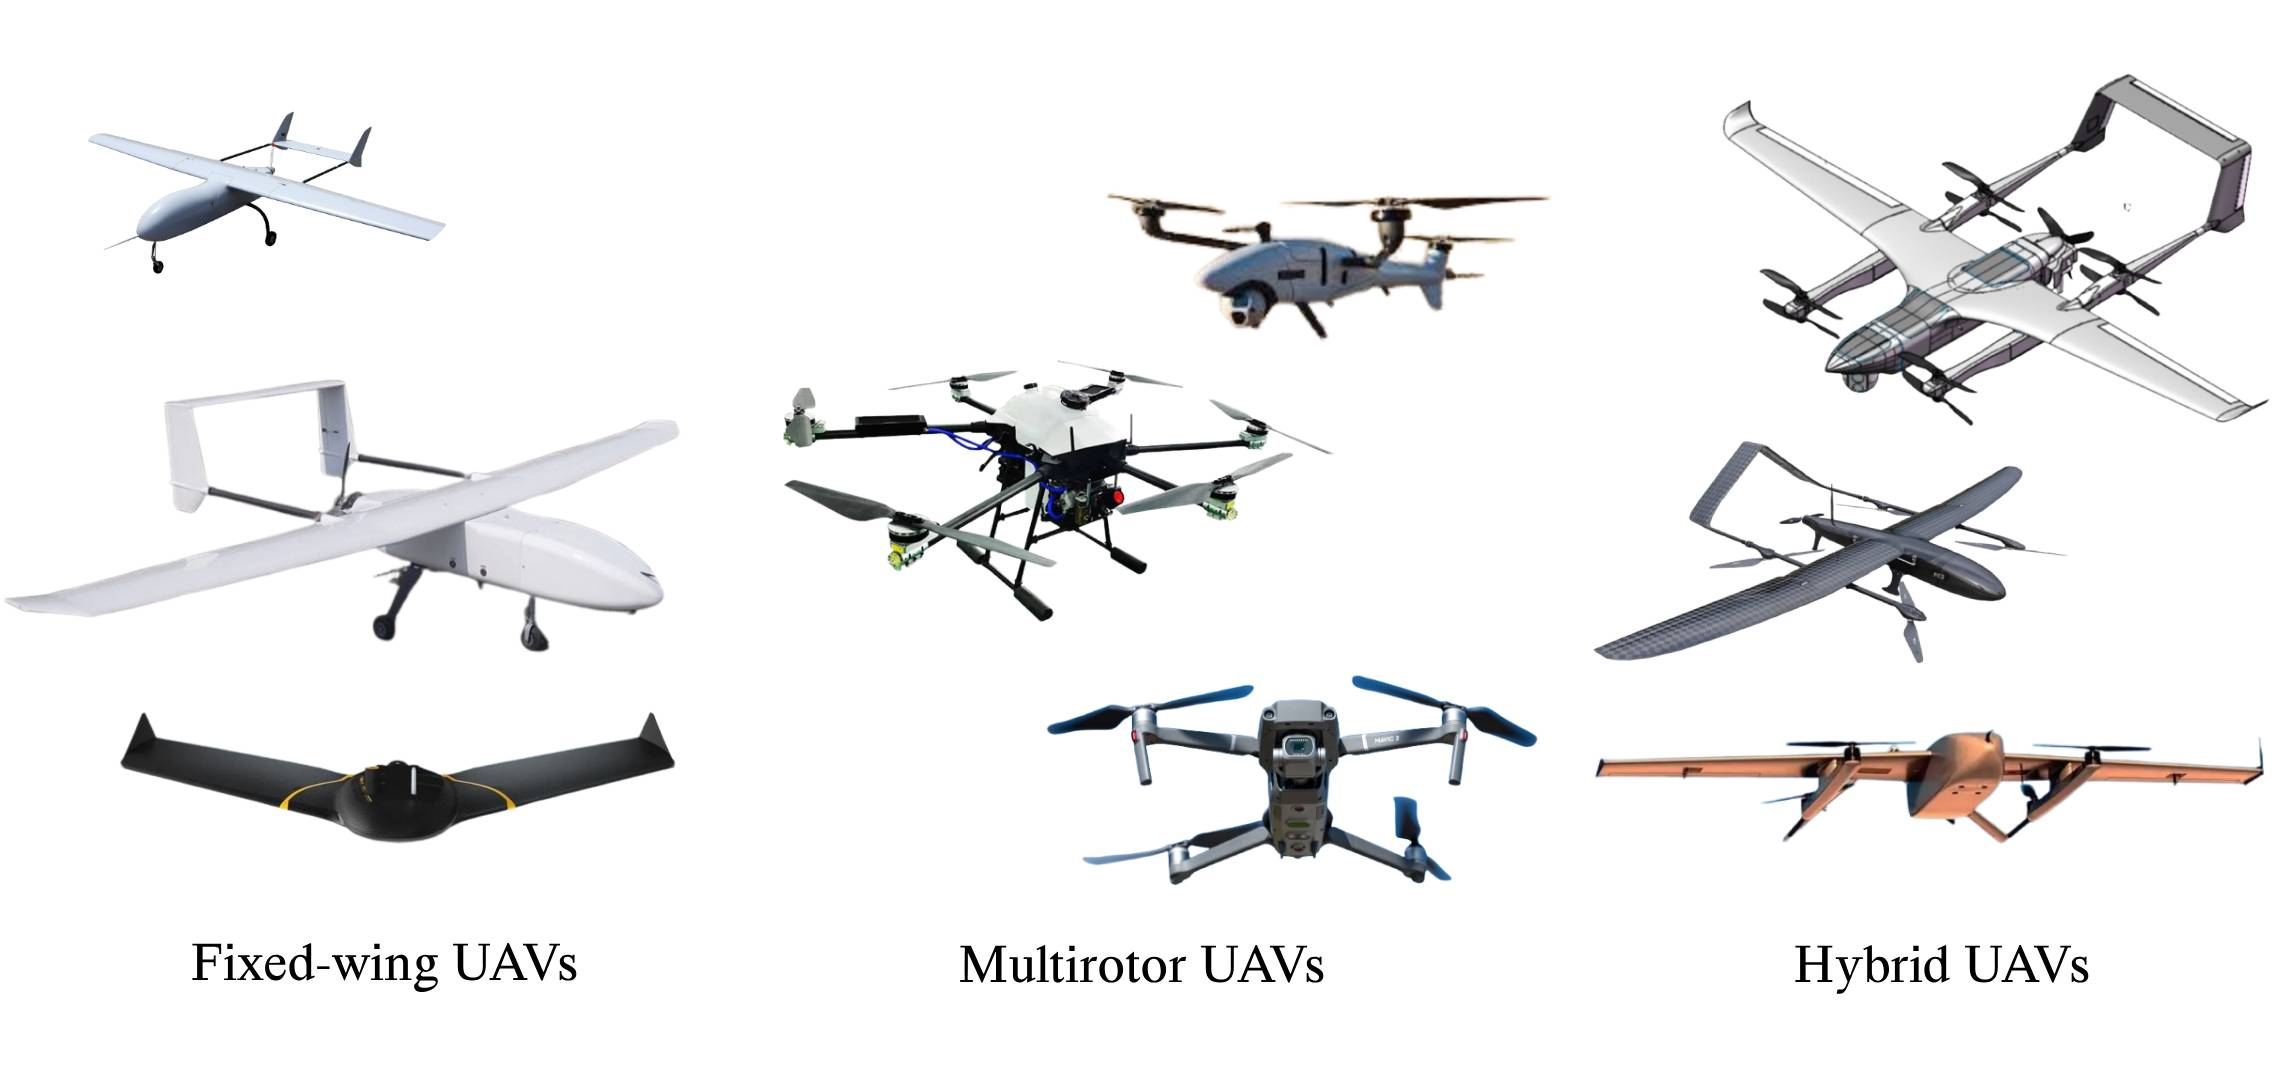
\includegraphics[width=14cm]{figure1/UAVs_types.jpg}
    \caption{Classification of UAV types. \label{UAVs_types}}
\end{figure}

% --- Section 1.2: Focus on Rotorcraft Platforms ---
\section{Focus on Rotorcraft Platforms}
\label{sec:intro_platforms}

This thesis focuses on the control of three distinct and challenging rotorcraft configurations, each selected to address different facets of the control problem.



\subsection{UAVs with Two Rotors}
UAVs with two rotors, characterized by perpendicular rotation axes, serve as a primary benchmark for this research, as depicted in Figure~\ref{UAVs2rotors}. These systems are designed to emulate the complex dynamics of a helicopter, typically featuring a main rotor for pitch (vertical) motion and a tail rotor for yaw (horizontal) motion. This configuration is characterized by its highly coupled, inherently unstable, and nonlinear dynamics, making it an ideal testbed for validating the performance of advanced control strategies under demanding conditions  \cite{trms_review1,trms_review2}.

\begin{figure}
    \centering
    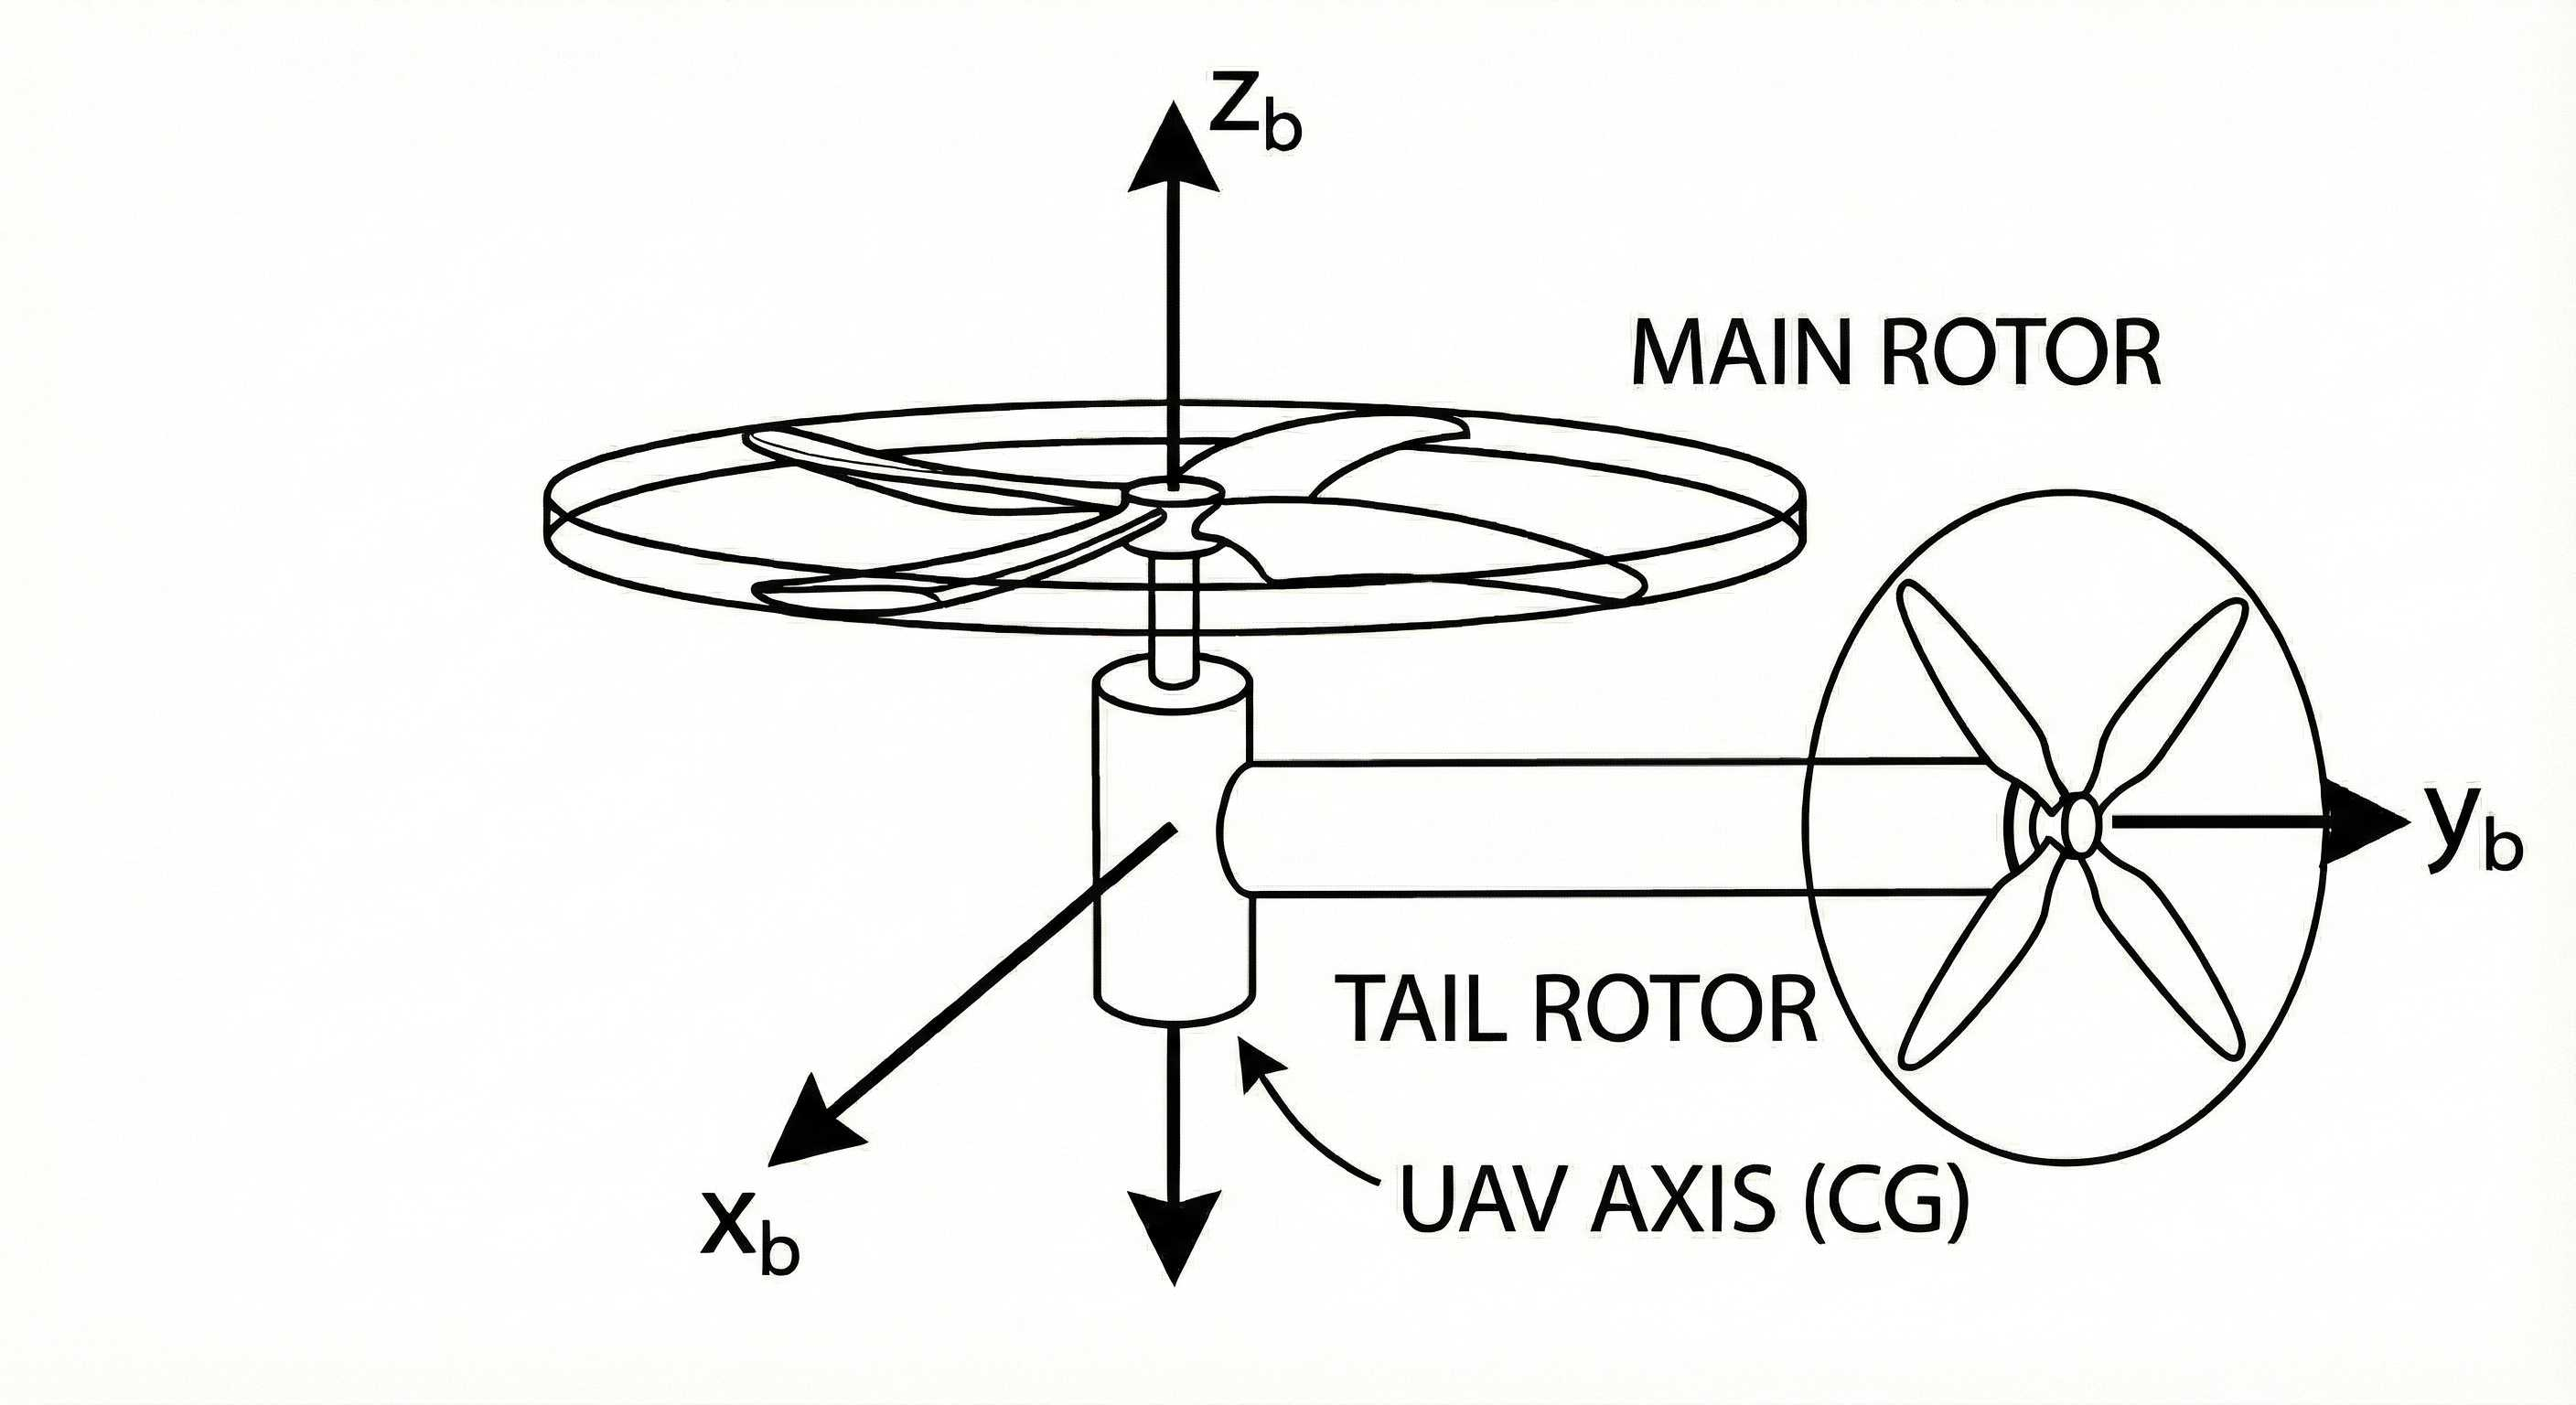
\includegraphics[width=10cm]{figure1/uav1.jpg}
    \caption{Basic UAV diagram with Two Rotors. \label{UAVs2rotors}}
\end{figure}

\subsection{Quadrotor UAV}
The quadrotor, as shown in Figure~\ref{quadrotor}, is one of the most common UAV configurations found in both academic research and commercial applications. Its mechanical design is simple, consisting of four rotors arranged in a cross formation, but this simplicity hides its complex six-degree-of-freedom (6-DOF) dynamics. The quadrotor is popular due to its high agility and maneuverability. However, achieving stable and precise trajectory tracking requires controllers that can effectively manage its underactuated and nonlinear nature  \cite{quadrotor_review1,quadrotor_review2}.

\begin{figure}
    \centering
    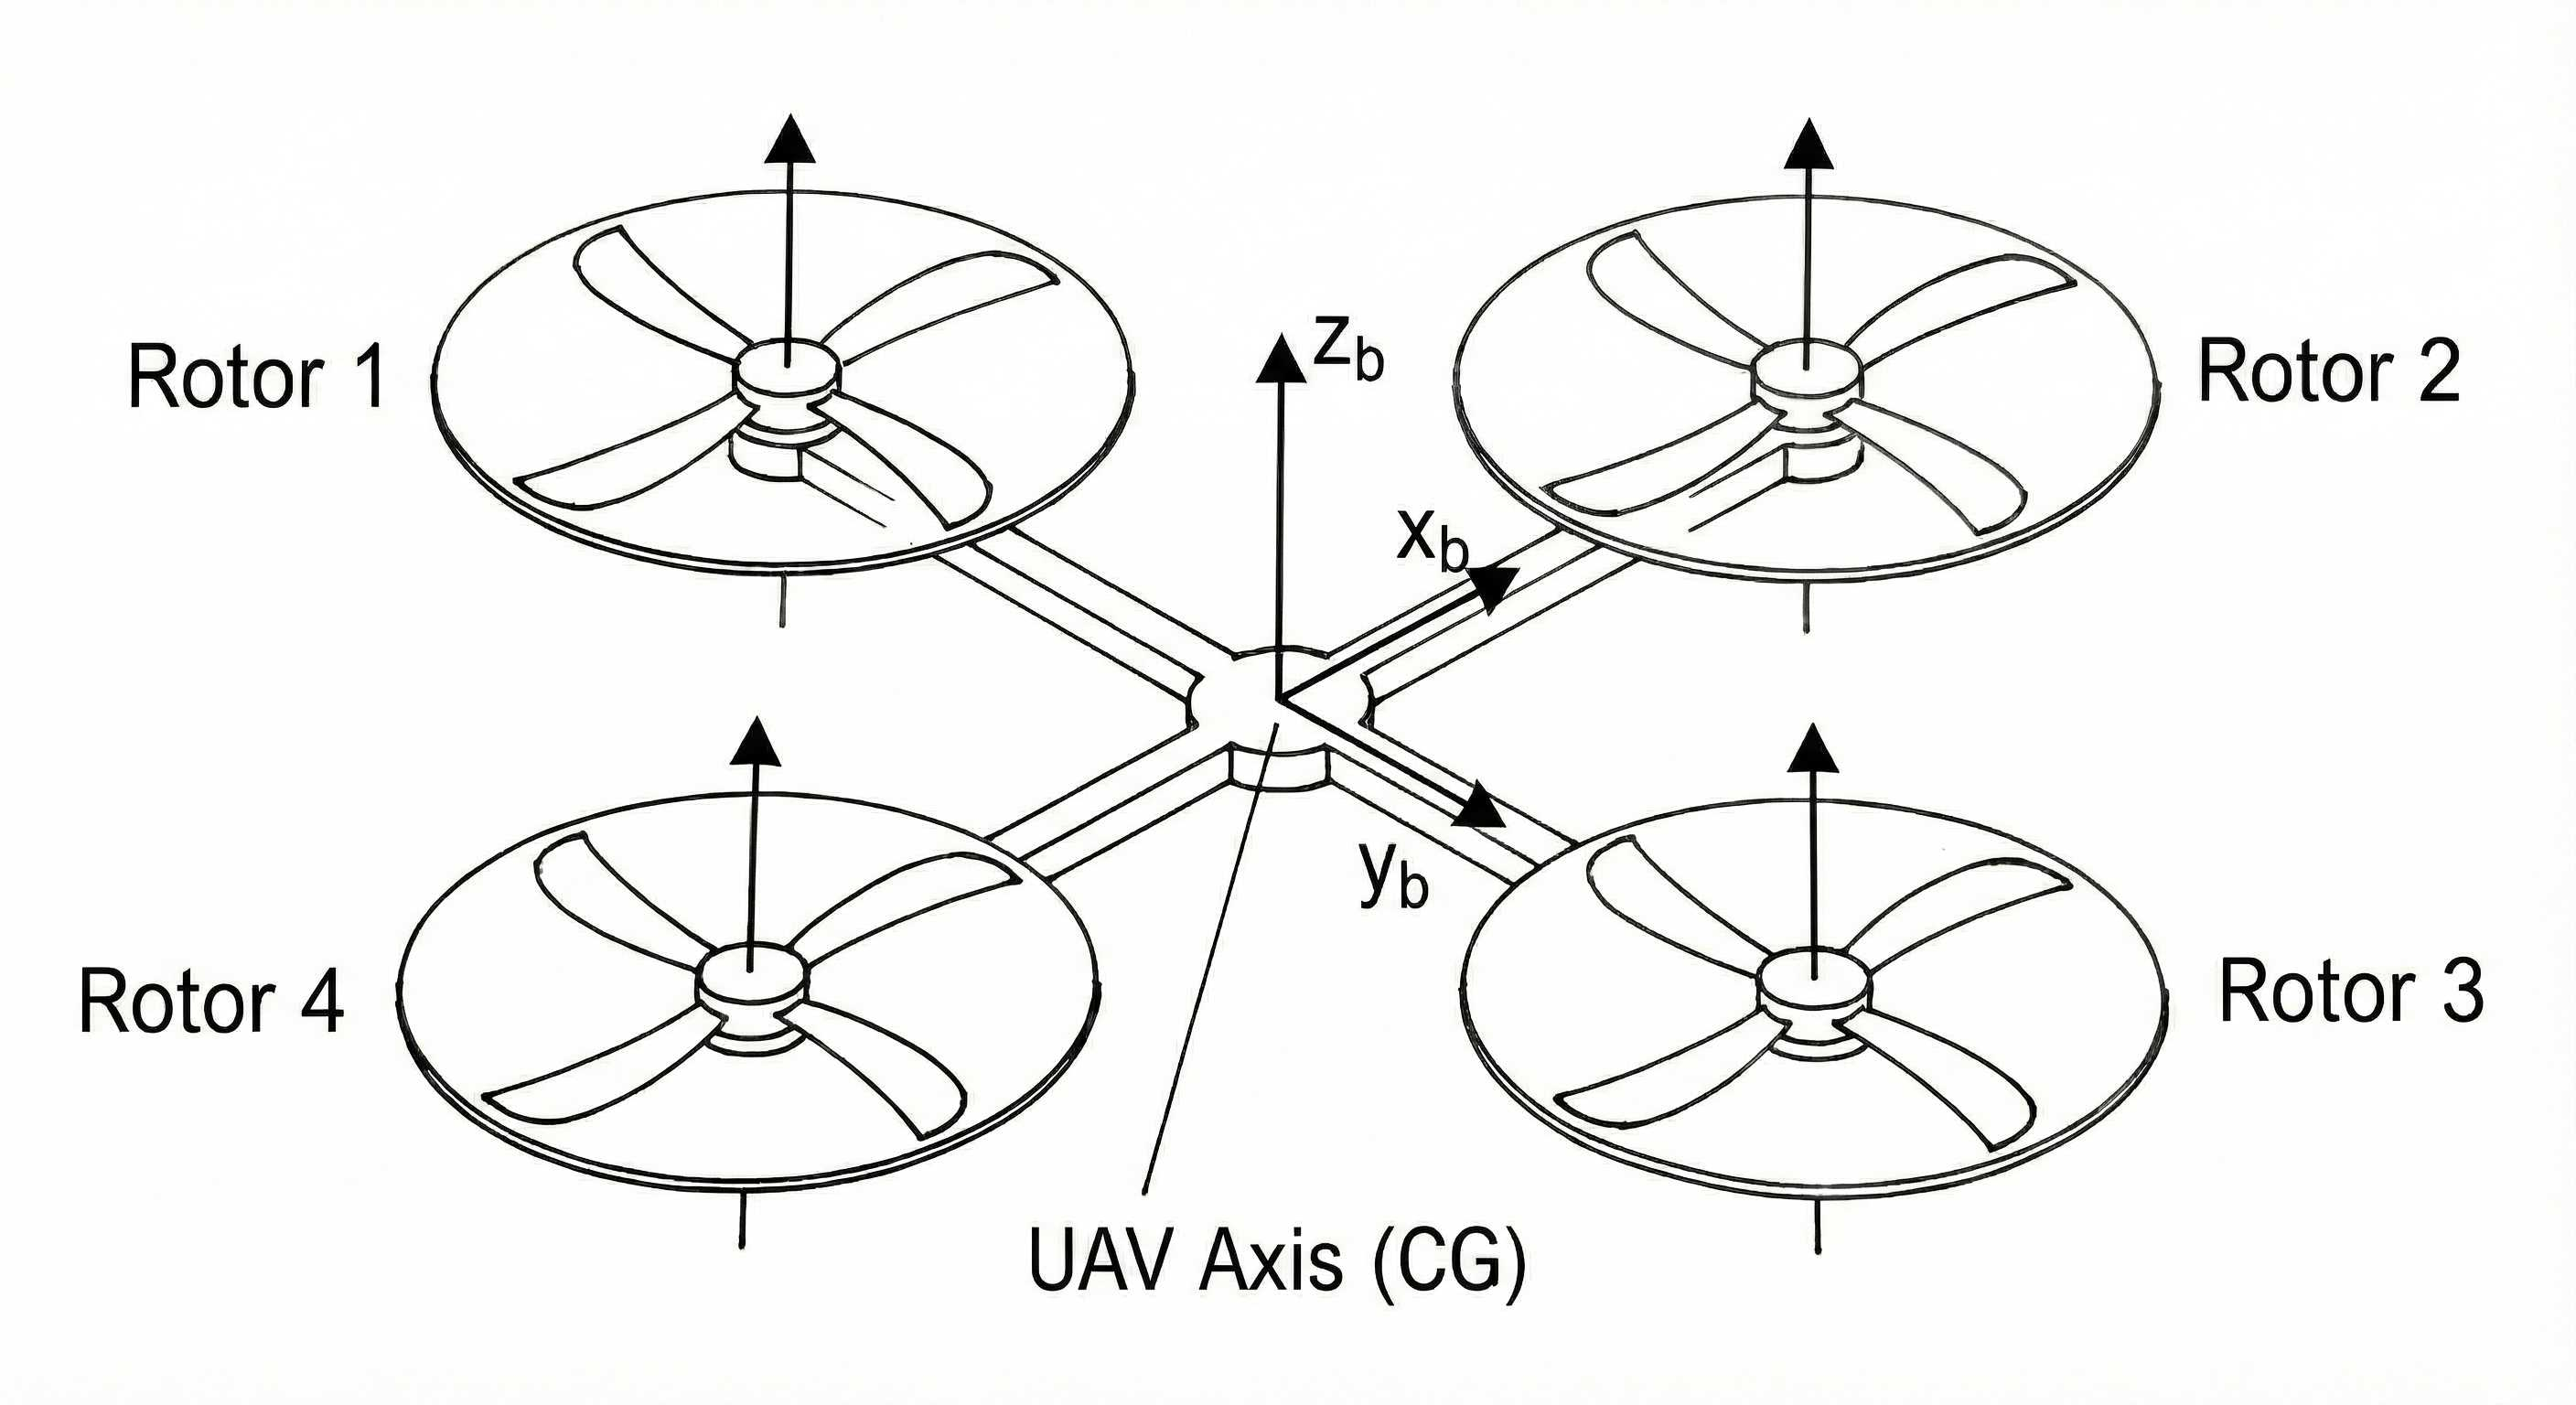
\includegraphics[width=10cm]{figure1/uav2.jpg}
    \caption{Basic quadrotor diagram. \label{quadrotor}}
\end{figure}

\subsection{Coaxial Rotor UAV}
The coaxial rotor configuration, shown in Figure~\ref{coaxial}, features two rotors stacked on the same axis that rotate in opposite directions. This setup offers a compact design with a high lift capacity for its size. A major benefit of this design is that the counter-rotating rotors cancel out each other's torque, which removes the need for a tail rotor and allows for a simpler, more streamlined body. While this is an advantage, the airflow from the top rotor directly affects the bottom rotor, creating complex aerodynamic interactions. These interactions introduce significant challenges for control, often requiring advanced control strategies to ensure stable and reliable performance  \cite{coaxial_review1,coaxial_review2,coaxial_review3}.

\begin{figure}
    \centering
    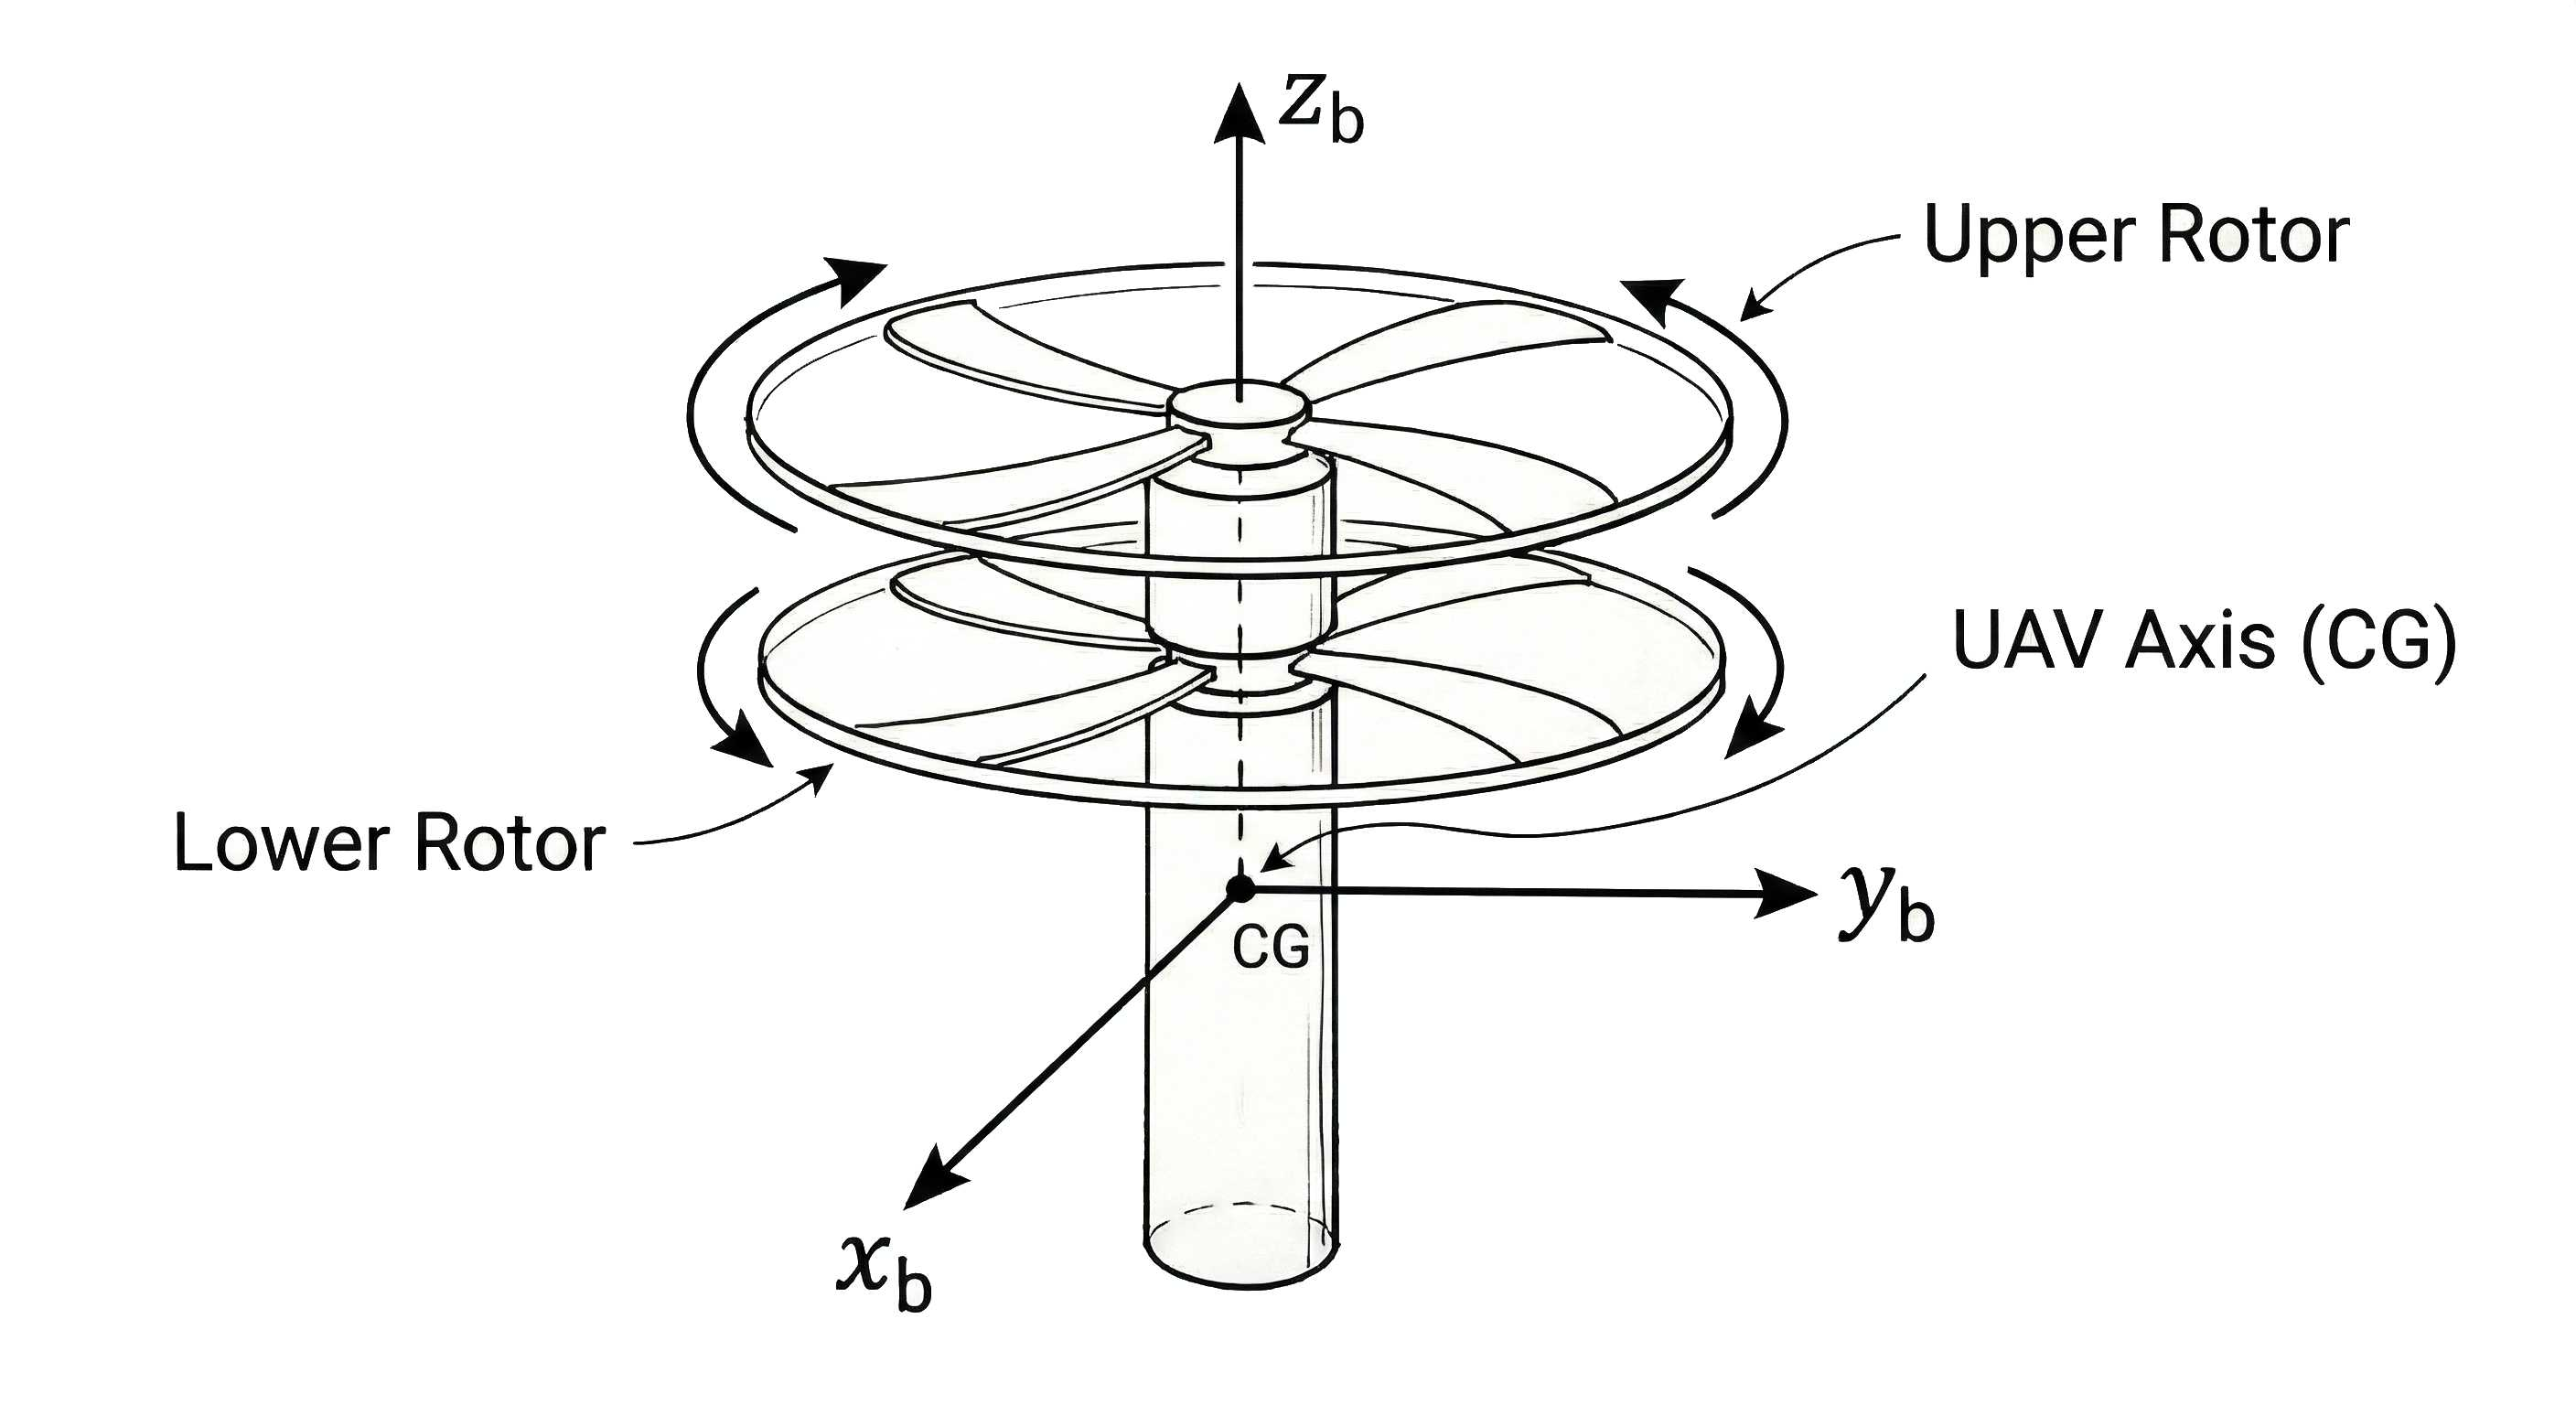
\includegraphics[width=10cm]{figure1/uav3.jpg}
    \caption{Basic coaxial UAV diagram. \label{coaxial}}
\end{figure}

% --- Section 1.3: The Core Control Challenge ---

\section{Review of UAV Control Strategies}
\label{sec:review_control_strategies}

The control of Unmanned Aerial Vehicles (UAVs) is a rich and diverse field, with a wide array of strategies developed to address their inherent dynamic challenges. The choice of controller is critical, as it directly dictates the vehicle's stability, performance and ability to execute complex missions. This section reviews the primary categories of control techniques applied to UAVs  \cite{control_methods}.

\subsection{Classical and Model-Based Control Methods}

Classical control strategies, which are primarily linear and rely on an explicit mathematical model of the system, represent the foundational layer of control design for UAVs. While often limited by their linear assumptions, their principles are well-understood, and they serve as an essential baseline for evaluating the performance of more advanced nonlinear and adaptive controllers.

Proportional-Integral-Derivative (PID) Control is the most widely used control algorithm in engineering, valued for its simplicity, intuitive tuning, and low computational cost  \cite{PID1,PID2}. The control law is formulated as a weighted sum of three terms: the present error (Proportional), the accumulation of past errors (Integral), and the prediction of future errors (Derivative). Mathematically, this is expressed as:
\begin{equation}
    u(t) = K_p e(t) + K_i \int_0^t e(\tau) \,d\tau + K_d \frac{de(t)}{dt}
\end{equation}
In this equation, $u(t)$ represents the control signal generated at time $t$. The variable $K_p$ denotes the proportional gain, which reacts to the current error $e(t)$, defined as the difference between the desired setpoint and the actual system state. $K_i$ is the integral gain, which acts on the accumulated error over time (where $\tau$ is the variable of integration), eliminating steady-state error. Finally, $K_d$ is the derivative gain, which scales the rate of change of the error $\frac{de(t)}{dt}$ to improve transient response and reduce overshoot. While effective for stabilization around a single operating point, the fixed gains of a PID controller cannot adapt to the UAV's changing dynamics across its flight envelope  \cite{PID3}.

Linear Quadratic Regulator (LQR) is an optimal control technique based on a linear state-space representation of the system dynamics, given by:
\begin{equation}
    \dot{x} = Ax + Bu
\end{equation}
where $\dot{x}$ is the time derivative of the state vector, $A$ is the system matrix describing the internal dynamics, $x$ represents the state vector, $B$ is the input matrix, and $u$ is the control input vector. The LQR algorithm computes a state-feedback gain matrix $K$ that minimizes a quadratic cost function $J$, defined as:
\begin{equation}
    J = \int_0^\infty (x^T Q x + u^T R u) dt
\end{equation}
where $J$ represents the scalar cost to be minimized over an infinite time horizon. The matrix $Q$ is a positive semi-definite state weighting matrix that penalizes deviations of the state $x$ from the equilibrium. The matrix $R$ is a positive definite control weighting matrix that penalizes the expenditure of control energy $u$. The resulting optimal control law is given by $u = -Kx$. LQR is naturally suited for the multi-input, multi-output (MIMO) nature of UAVs, but its performance is limited by its reliance on an accurate linear model  \cite{lqr1,lqr2}.

Model Predictive Control (MPC) is an advanced optimal control strategy that uses an explicit plant model to predict the system's future behavior over a finite time horizon, denoted as $N$. At each time step $k$, MPC solves an online optimization problem to find an optimal sequence of control inputs $U = \{u_k, u_{k+1}, \dots, u_{k+N-1}\}$ that minimizes a cost function $J$ while adhering to system constraints  \cite{mpc1,mpc2}. A key advantage of MPC for UAVs is its ability to explicitly handle operational constraints, such as actuator saturation (e.g., maximum motor speeds $u_{\min} \le u \le u_{\max}$) and state limits. Its primary drawback is the high computational burden of solving the optimization problem at every time step.

H-infinity ($H_{\infty}$) control is a robust control technique designed to minimize the effect of external disturbances and model uncertainties. The design objective is to find a controller that minimizes the "worst-case" gain from an exogenous input (like a wind gust) to a performance output (like a tracking error). This gain is measured by the $H_{\infty}$ norm of the system's transfer function. The goal is to ensure this norm remains below a specified level, guaranteeing robust stability and performance despite model inaccuracies. This makes $H_{\infty}$ control particularly suitable for UAVs, where the precise aerodynamic model is often unknown and the operating environment is unpredictable  \cite{hinf1,hinf2,hinf3}.

\subsection{Nonlinear Control Methods}
To overcome the inherent limitations of linear controllers, which are only valid around a specific operating point, a variety of nonlinear control strategies have been developed. These methods are designed to explicitly handle the complex, coupled, and highly nonlinear dynamics of rotorcraft across their entire flight envelope, providing superior performance and stability.

Feedback Linearization is a powerful technique that aims to algebraically transform a nonlinear system's dynamics into an equivalent linear one through a change of coordinates and nonlinear state feedback. Once the system is linearized, the full suite of well-established linear control techniques, such as LQR or PID, can be applied to the transformed system to achieve the desired performance. The primary advantage of this method is its ability to achieve precise control over the nonlinear system  \cite{fbl1,fbl2,fbl3}. However, its major drawback is a critical reliance on an exact and accurate mathematical model of the system. Any model uncertainties or external disturbances can lead to imperfect cancellation of the nonlinearities, severely degrading performance and potentially causing instability.

Backstepping Control is a recursive and systematic design methodology for a specific class of nonlinear systems known as "strict-feedback" or "triangular" systems. It is particularly well-suited for high-order systems, as it breaks down the complex control design problem into a sequence of smaller, more manageable steps. Starting from the known stable subsystem, it recursively designs a "virtual control" law for each subsequent subsystem, treating the error from the previous step as a new state. At each step, a Lyapunov function is augmented to prove the stability of the extended subsystem. This process continues until the final step, where the actual control input is designed \cite{bsc1,bsc2,bsc3}. The backstepping technique is powerful for its ability to guarantee stability and performance for a broad class of nonlinear systems and serves as the foundational framework for the controllers developed in this thesis.

Sliding Mode Control (SMC) is a highly robust control technique renowned for its excellent disturbance rejection properties and insensitivity to matched parameter variations and uncertainties. The design involves two phases. First, a sliding surface (or manifold) is defined in the state space, which represents the desired system dynamics. Second, a discontinuous control law is designed to drive the system's state trajectories onto this surface in finite time (the "reaching phase") and maintain them there for all subsequent time (the "sliding phase"). While on the surface, the system's behavior is dictated by the surface's design and is invariant to certain classes of disturbances. While exceptionally robust, a key drawback of conventional SMC is the chattering phenomenon. This refers to high-frequency oscillations in the control signal caused by the rapid switching required to keep the states on the sliding surface. Chattering is undesirable as it can excite unmodeled high-frequency dynamics and cause excessive wear or damage to actuators  \cite{smc1,smc2,smc3}.

\subsection{Model-Free and Intelligent Control Techniques}
A significant challenge in the design of high-performance controllers is the inherent reliance on an accurate mathematical model of the system. For UAVs, creating such a model is exceptionally difficult due to complex aerodynamics, unmodeled dynamics (e.g., ground effect, blade flapping), and time-varying parameters (e.g., battery discharge, payload changes). To overcome this, Model-Free Control offers a powerful alternative paradigm. Instead of relying on a predefined physical model, MFC strategies use real-time input and output data to estimate the system's behavior through a continuously updated, "ultra-local" model  \cite{mfc1,mfc2,mfc3}. This approach effectively treats the complex plant as a simpler system whose dynamics are learned or approximated online. Intelligent techniques are among the most effective methods for this purpose, thereby reducing the dependency on a precise model.

\begin{itemize}
    \item \textbf{Neural Network (NN) Control:} NNs, particularly Radial Basis Function Neural Networks (RBFNN), are used as universal function approximators. They can learn the unknown nonlinear dynamics of a UAV in real-time, providing an adaptive component to the control law. This allows the controller to compensate for unmodeled dynamics and time-varying parameters  \cite{my1article}.

    \item \textbf{Fuzzy Logic Control (FLC):} Fuzzy Logic Systems (FLS) use linguistic `IF-THEN` rules to map inputs to outputs, mimicking human-like reasoning. They are highly effective at handling system uncertainties and nonlinearities without requiring a mathematical model. FLS are employed to adaptively estimate and compensate for unknown dynamics, disturbances and fault effects  \cite{my2article}.
\end{itemize}
These intelligent techniques are often integrated with nonlinear frameworks like backstepping or sliding mode control to combine the systematic stability of the latter with the adaptive capabilities of the intelligent component to handle all the system's unknown elements.

\section{Fault-Tolerant Control (FTC) Paradigms}
\label{sec:ftc_paradigms}
Fault-Tolerant Control  is a critical subfield of control engineering focused on maintaining system stability and acceptable performance in the event of component failures. A fault is defined as an unpermitted deviation of at least one characteristic property of the system from its nominal behavior  \cite{ftc1,ftc2,ftc3,ftc4}. The primary goal of an FTC system is to preserve the operational integrity of the UAV, preventing minor faults from escalating into catastrophic failures. FTC strategies are generally categorized into two main paradigms: passive and active.

\subsection{Passive FTC}
Passive Fault-Tolerant Control (PFTC) systems rely on the inherent robustness of a single, fixed-parameter controller. This controller is designed offline to be resilient to a predefined and limited set of potential faults  \cite{passive1}. The design strategy is to create a controller with a high degree of robustness to uncertainties, such that certain faults are treated as additional model uncertainties that the controller can handle without modification. Techniques like H-infinity control, quantitative feedback theory (QFT), and linear parameter-varying (LPV) control are often employed for this purpose \cite{passive2,passive3,passive4}.

While PFTC systems are simpler to implement as they do not require an online fault diagnosis mechanism, they have significant limitations. They are inherently conservative, as the controller must be robust enough to handle the worst-case fault scenario, which can lead to suboptimal performance under nominal (fault-free) conditions. Most critically, their performance degrades significantly when faced with unexpected faults or failures whose magnitudes exceed the anticipated design range.

\subsection{Active FTC}
Active Fault-Tolerant Control (AFTC) systems, in contrast, employ a dynamic and adaptive approach to handling faults. An AFTC system is designed to explicitly detect, diagnose and react to faults in real-time by reconfiguring the control strategy to accommodate the fault's effects. This adaptability allows AFTC to handle a much wider range of unforeseen faults and maintain a higher level of performance post-fault  \cite{active1,active2,active3}.

The core of an AFTC system is an online Fault Detection and Diagnosis (FDD) module. The FDD process is typically sequential and consists of three stages  \cite{fdd1,fdd2}:

\begin{enumerate}
    \item \textbf{Fault Detection:} This initial stage involves determining whether a fault has occurred in the system. This is commonly achieved by generating and monitoring a \textit{residual} signal, which represents the discrepancy between the measured system output and the output predicted by a nominal model  \cite{Isermann2011, ftc_UAV_review2}. When the residual exceeds a predefined threshold often determined via statistical methods to account for sensor noise a fault is declared  \cite{active1}.
    
    \item \textbf{Fault Isolation:} Once a fault is detected, this stage determines its precise location (e.g., distinguishing between a failure in the front-right motor versus the onboard IMU sensor)  \cite{Scognamiglio2024}.
    
    \item \textbf{Fault Identification:} This final stage estimates the characteristics of the fault, such as its magnitude, severity and time-variant behavior (e.g., abrupt, incipient, intermittent)  \cite{Zhang2008, Liu2022}.
\end{enumerate}

Based on the information provided by the FDD module, the AFTC system then performs fault accommodation by adjusting the control law. This can involve retuning controller gains, switching to a different control algorithm, or reconfiguring the control allocation to redistribute control effort among the remaining healthy actuators  \cite{Alwi2024, Steinberg2021}.

\section{Intelligent Function Approximators}
\label{sec:intelligent_approximators}

Accurate mathematical modeling of complex nonlinear systems is often intractable due to unmodeled dynamics and external disturbances. To address this, intelligent function approximators, specifically Radial Basis Function Neural Networks (RBFNN) and Fuzzy Logic Systems (FLS), are employed for their robust, model-free estimation capabilities. Supported by the Universal Approximation  \cite{universal}, these techniques can approximate any continuous nonlinear function to an arbitrary degree of accuracy on a compact set without requiring knowledge of the physical system parameters. Extensive literature demonstrates their superiority over classical approximation methods, such as Time Delay Estimation (TDE) and Chebyshev polynomials \cite{chebyshev,coaxial_review3}.

\subsection{Radial Basis Function Neural Networks }

A Radial Basis Function Neural Network (RBFNN) is a type of feedforward artificial neural network highly valued in adaptive control for its ability to model complex nonlinear dynamics. RBFNNs are recognized as universal approximators, meaning that with a sufficient number of neurons in the hidden layer, they can approximate any continuous nonlinear function $\mathcal{H}(\mathbf{Z})$ on a compact set to any desired degree of accuracy  \cite{rbfnn1,rbfnn2}.

As illustrated in Figure \ref{fig:rbfnn_arch}, the architecture of an RBFNN is structurally simple, consisting of three distinct layers interacting sequentially: an input layer, a single nonlinear hidden layer, and a linear output layer.

\begin{figure}[htbp]
    \centering    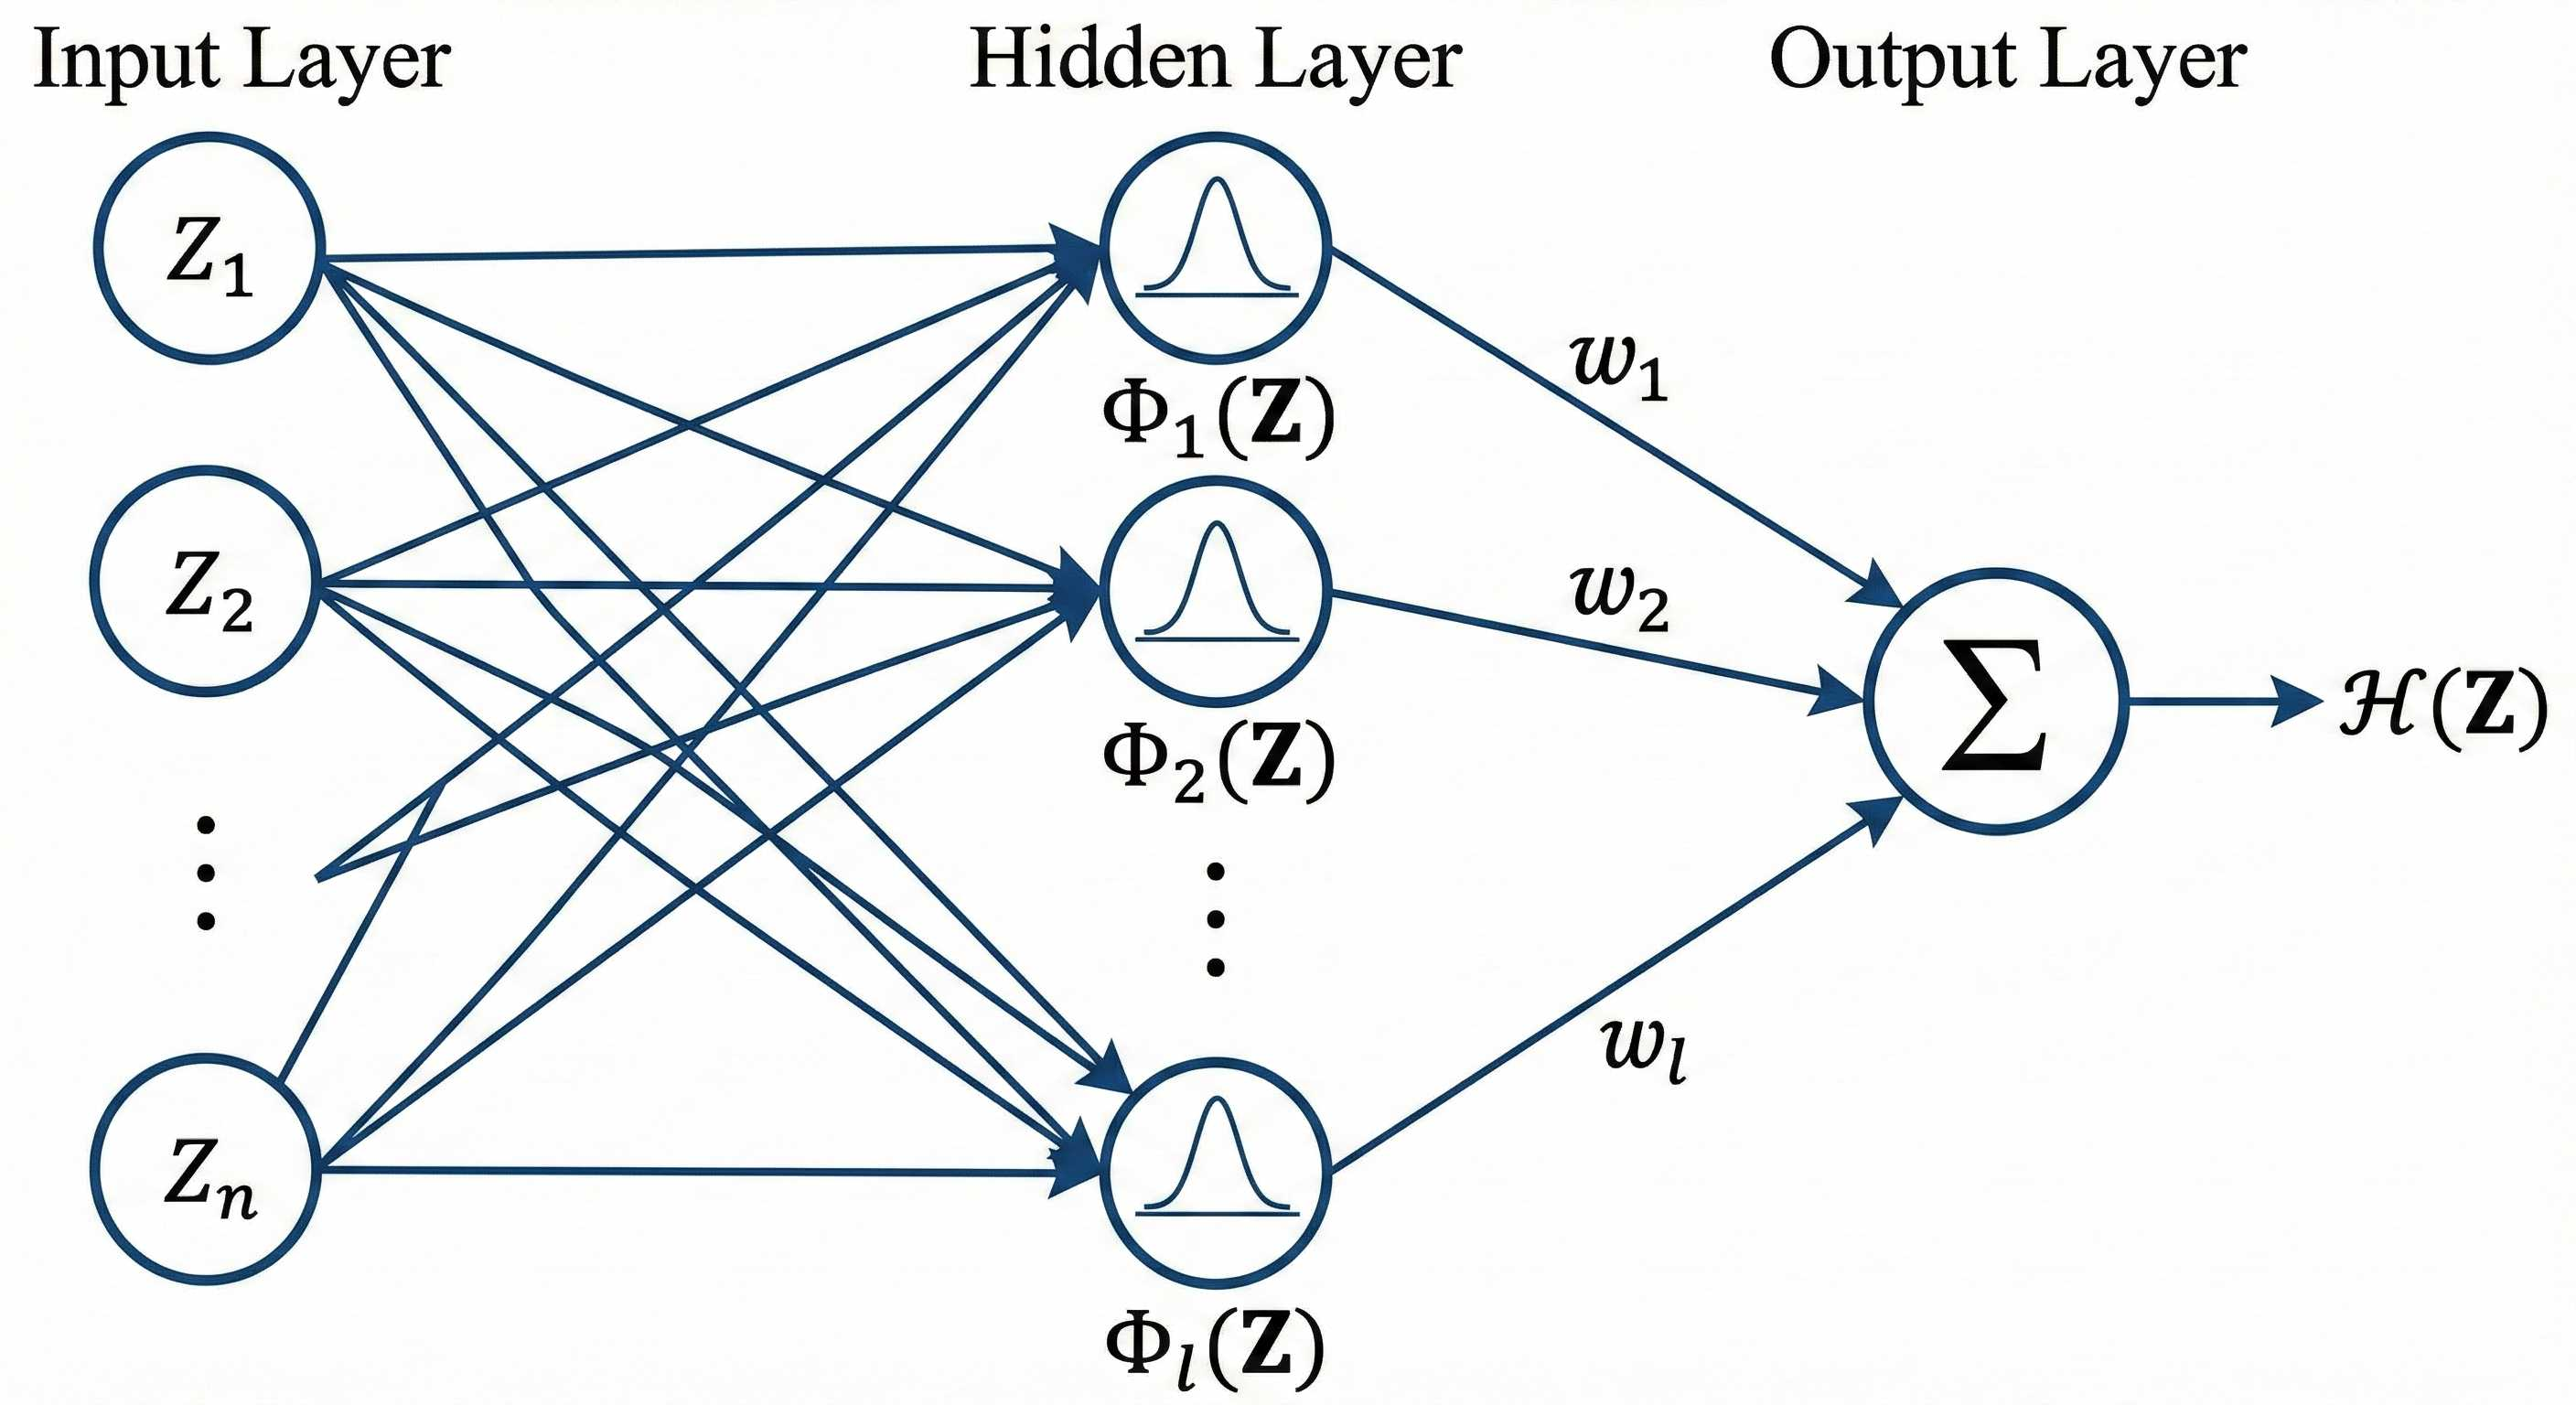
\includegraphics[width=0.6\linewidth]{figure2/rbfnn_architecture.jpg}
    \caption{Schematic diagram of a three-layer Radial Basis Function Neural Network architecture.}
    \label{fig:rbfnn_arch}
\end{figure}

The process begins at the input layer, which receives the input vector $\mathbf{Z}~=~[z_1, z_2, \dots, z_n]^T \in \mathbb{R}^n$, where $n$ denotes the dimensionality of the input state or environmental variables. The nodes in this layer do not perform any computation; their sole purpose is to transmit these input signals directly to the subsequent hidden layer neurons.

Following the input stage is the hidden layer, which acts as the core processing unit of the network. The activation of each hidden neuron is determined by a radial basis function. The most commonly used choice is the \textbf{Gaussian function}, defined for the $i$-th hidden neuron as:
\begin{equation}
    \phi_i(\mathbf{Z}) = \exp\left(-\frac{\|\mathbf{Z} - \mathbf{\mu_i}\|^2}{\eta_i^2}\right)
\end{equation}
In this equation, $\phi_i(\mathbf{Z})$ represents the activation output of the $i$-th neuron. $\mathbf{\mu_i} \in \mathbb{R}^n$ is the center vector for that specific neuron, representing the point in the input space where activation is maximized. The parameter $\eta_i$ represents the width of the Gaussian function, which determines the neuron's "receptive field" or sensitivity to inputs as they deviate from the center.

The final layer performs a linear computation to generate the network's output. The output of the RBFNN is formed by a weighted linear combination of the activation values received from the hidden layer. Mathematically, the network's approximation of the function $\mathcal{H}(\mathbf{Z})$ is expressed as:
\begin{equation}
    \mathcal{H}(\mathbf{Z}) = \mathbf{W}^T \Phi(\mathbf{Z}) + \delta(\mathbf{Z})
    \label{eq:rbfnn_approx}
\end{equation}
where $\mathbf{W} = [w_1, w_2, \dots, w_l]^T \in \mathbb{R}^l$ is the vector of ideal network weights connecting the hidden layer to the output layer. The scalar $l$ denotes the total number of neurons (or nodes) in the hidden layer. $\Phi(\mathbf{Z}) = [\phi_1(\mathbf{Z}), \phi_2(\mathbf{Z}), \dots, \phi_l(\mathbf{Z})]^T \in \mathbb{R}^l$ is the regressor vector containing the radial basis function outputs. Finally, $\delta(\mathbf{Z})$ represents the inherent approximation error, which is guaranteed to be bounded such that $|\delta(\mathbf{Z})| \le \epsilon$, where $\epsilon$ is a small positive constant. In adaptive control scenarios, the ideal weights $\mathbf{W}$ are typically unknown and must be estimated online using an appropriate adaptation law.

\subsection{Fuzzy Logic Systems }

A Fuzzy Logic System (FLS) is an intelligent control methodology that leverages the principles of fuzzy set theory to handle uncertainty and imprecision, effectively mimicking human-like reasoning  \cite{zadeh1965}. Unlike classical control strategies that rely on rigid binary logic, FLS processes information using degrees of truth, making it exceptionally well-suited for the control of UAVs where dynamic models are often complex or vulnerable to faults.

In the literature, two primary types of fuzzy inference systems are widely recognized: the Mamdani  \cite{mamdani1974} and the Takagi-Sugeno-Kang (TSK)  \cite{takagi1985} models. The Mamdani model is characterized by the use of fuzzy sets in the rule consequents, making it highly intuitive for capturing expert human knowledge. In contrast, the Takagi-Sugeno model employs deterministic functions as rule consequents, which is generally more computationally efficient. This thesis utilizes a structure that aligns with the efficiency of the Sugeno model while retaining the interpretability of fuzzy basis functions.

As illustrated in Figure \ref{fig:fls_arch}, the architecture of an FLS is structurally similar to that of a neural network, processing information sequentially through fuzzification, inference, and defuzzification.

\begin{figure}[htbp]
    \centering
    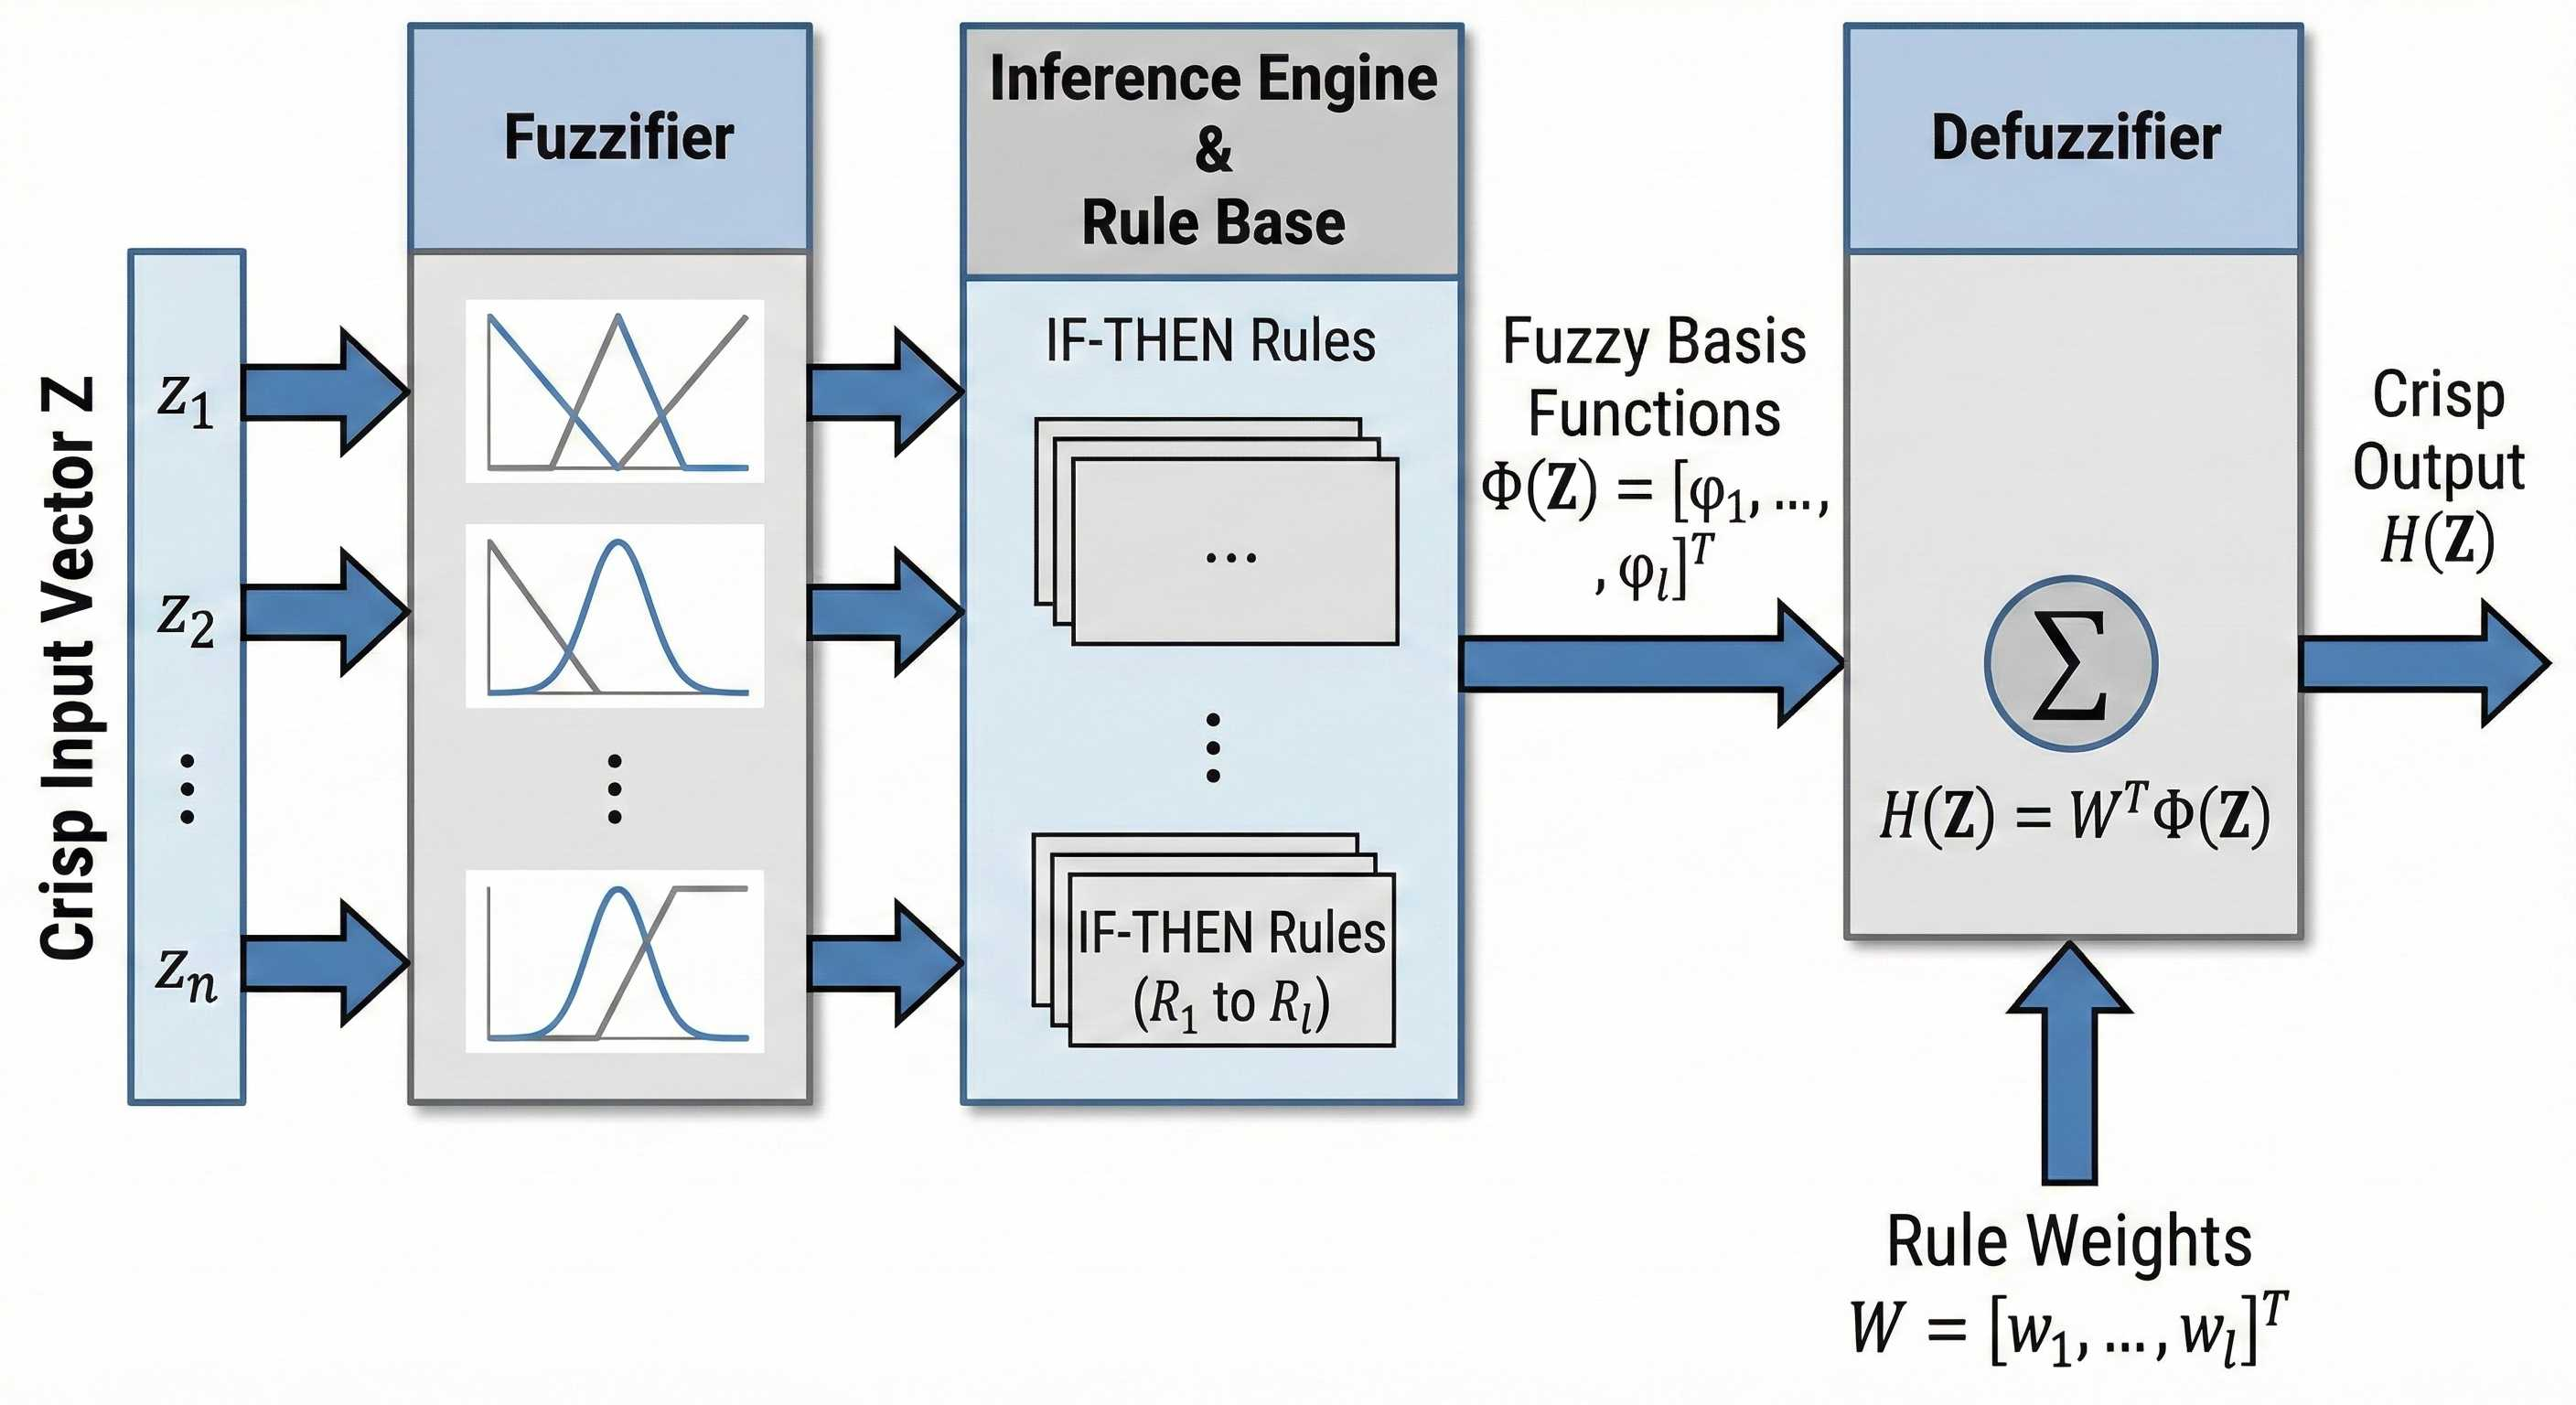
\includegraphics[width=0.8\linewidth]{figure2/fls_architecture.jpg}
    \caption{Schematic diagram of the Fuzzy Logic System architecture.}
    \label{fig:fls_arch}
\end{figure}

The process begins with the input vector $\mathbf{S} = [s_1, s_2, \dots, s_n]^T \in \mathbb{R}^n$, where $n$ denotes the dimensionality of the input state or environmental variables. These crisp inputs are mapped to fuzzy sets using membership functions.

Following the input stage is the inference engine, which acts as the core processing unit. Analogous to the hidden layer of a neural network, it evaluates a set of `IF-THEN` rules. The activation of each rule is determined by the fuzzy basis function. For the $i$-th rule, the normalized firing strength $\psi_i(\mathbf{S})$ is defined as:
\begin{equation}
    \psi_i(\mathbf{S}) = \frac{\prod_{j=1}^{n} \mu_{F_j^i}(s_j)}{\sum_{k=1}^{l} \left( \prod_{j=1}^{n} \mu_{F_j^k}(s_j) \right)}
\end{equation}
In this equation, $\mu_{F_j^i}(s_j)$ represents the membership degree of the input $s_j$ to the fuzzy set $F_j^i$.

The final stage performs a computation to generate the system's output. The output of the FLS is formed by a weighted linear combination of the fuzzy basis functions. By leveraging the universal approximation property  \cite{wang1992}, the FLS approximation of the continuous nonlinear function $\mathcal{F}(\mathbf{S})$ is expressed as:
\begin{equation}
    \mathcal{F}(\mathbf{S}) = \boldsymbol{\Theta}^T \Psi(\mathbf{S}) + \zeta(\mathbf{S})
    \label{eq:fls_approx}
\end{equation}
where $\boldsymbol{\Theta} = [\theta_1, \theta_2, \dots, \theta_l]^T \in \mathbb{R}^l$ is the vector of adjustable rule consequent parameters (weights). The scalar $l$ denotes the total number of fuzzy rules. $\Psi(\mathbf{S}) = [\psi_1(\mathbf{S}), \psi_2(\mathbf{S}), \dots, \psi_l(\mathbf{S})]^T \in \mathbb{R}^l$ is the regressor vector containing the fuzzy basis function outputs. Finally, $\zeta(\mathbf{S})$ represents the inherent approximation error, which is guaranteed to be bounded such that $|\zeta(\mathbf{S})| \le \epsilon$, where $\epsilon$ is a small positive constant. In adaptive control scenarios, the ideal weights $\boldsymbol{\Theta}$ are typically unknown and must be estimated online using an appropriate adaptation law.







\subsection{Universal Approximation Theorem}
\label{sec:universal_approximation}

The Universal Approximation Theorem states that intelligent RBFNN and FLS, can approximate any continuous nonlinear function on a compact domain to an arbitrary degree of accuracy. 

In this thesis, this theorem provides the rigorous theoretical justification for employing RBFNNs and FLS to online estimate unknown nonlinear dynamics, external aerodynamic disturbances, and sensor or actuator faults. By guaranteeing a bounded approximation error, it serves as a fundamental prerequisite for proving the fixed-time stability and robustness of the proposed fault-tolerant control laws.

The theorem can be formally stated as follows:

\textbf{Theorem (Universal Approximation):} Let $\mathcal{H}(\mathbf{Z}): \Omega \rightarrow \mathbb{R}$ be a continuous real-valued function defined on a compact operating space $\Omega \subset \mathbb{R}^n$. For any arbitrarily small positive constant $\epsilon > 0$, there exists an ideal weight vector $\mathbf{W}^*$ and a set of basis functions $\Phi(\mathbf{Z})$ (such as radial basis functions or fuzzy basis functions) such that the following condition holds:
\begin{equation}
    \sup_{\mathbf{Z} \in \Omega} \left| \mathcal{H}(\mathbf{Z}) - \mathbf{W}^{*T} \Phi(\mathbf{Z}) \right| \leq \epsilon
\end{equation}
where $\mathbf{W}^{*T} \Phi(\mathbf{Z})$ represents the output of the approximator (RBFNN or FLS), and $\epsilon$ is the strictly bounded approximation error.\section{Key Theoretical Concept: Fixed-Time Stability}
\label{sec:fixed_time_stability}

Stability is the most fundamental requirement of any control system. However, in safety-critical applications such as autonomous UAVs, simply guaranteeing that the system will "eventually" stabilize is insufficient. The demanding nature of aerial maneuvers, especially in the presence of actuator faults or severe external disturbances, requires strict guarantees regarding the speed of convergence. This thesis elevates the stability requirement by focusing on \textbf{fixed-time stability}, a concept that offers stronger and more practical performance guarantees than traditional notions.

To understand the critical advantage of this approach, it is necessary to compare it with standard stability concepts. Figure \ref{fixed_time_comparison} provides a comparative illustration of the system trajectories under three distinct stability paradigms: asymptotic, finite-time, and fixed-time stability.

\begin{figure}[h!]
\centering
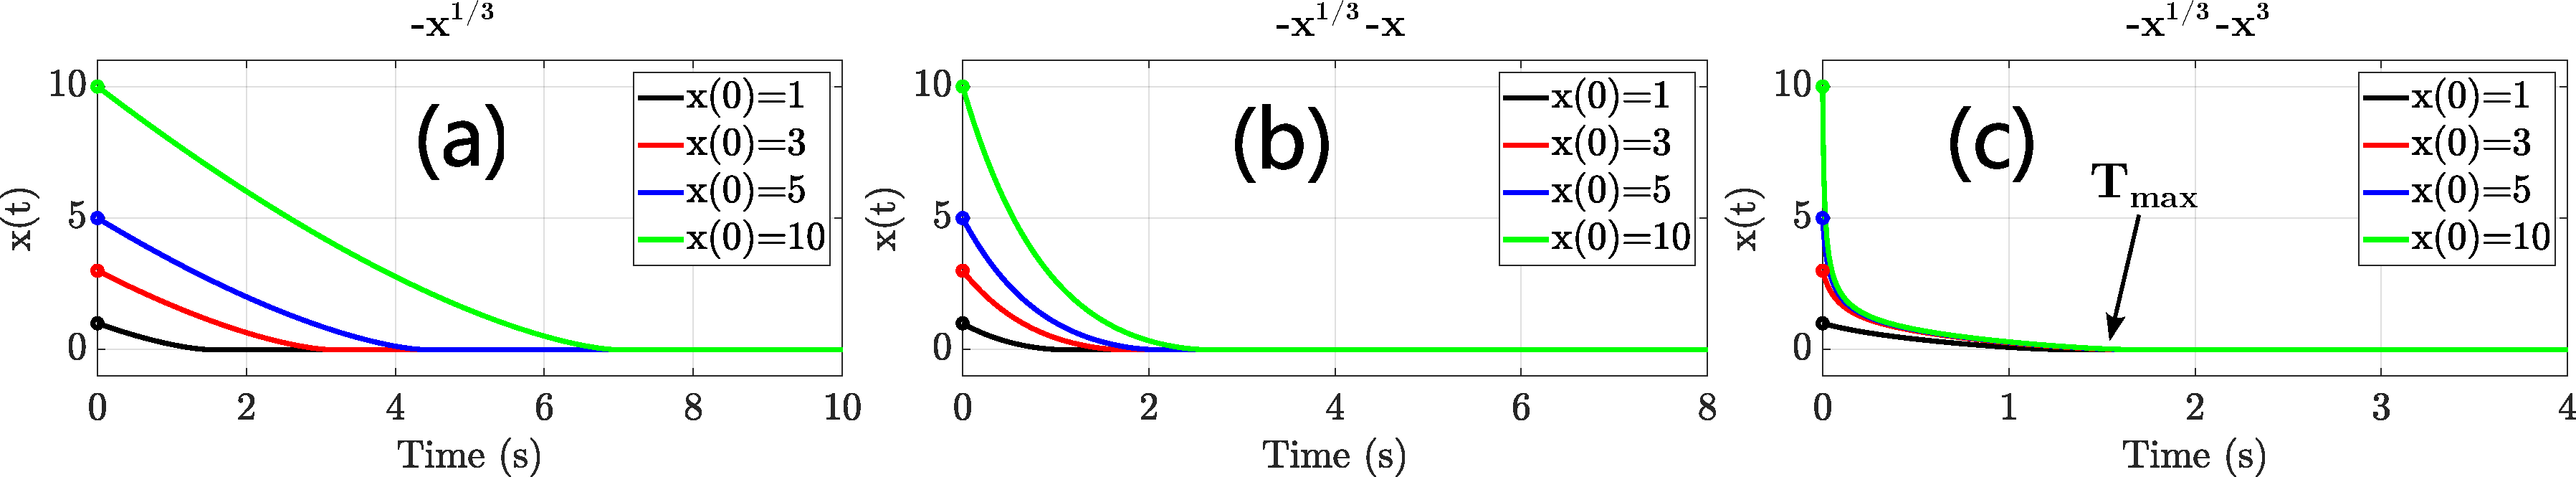
\includegraphics[width=14cm]{figure2/fixed time test.pdf}
\caption{Stability Comparison for Different Initial Conditions.}
\label{fixed_time_comparison}
\end{figure}

\begin{enumerate}
    \item \textbf{Asymptotic Stability:} 
    This is the standard form of stability found in classical linear control. As shown in Figure \ref{fixed_time_comparison}a, the system states approach the equilibrium (zero) gradually as time progresses towards infinity ($t \to \infty$). While the error decreases, it theoretically never reaches absolute zero in finite time. More critically, the time required to reach a specific "small enough" error neighborhood depends heavily on the initial condition. If a fault causes a large deviation (a large initial error), the system may take an unacceptably long time to recover, potentially leading to a crash before stability is regained.

    \item \textbf{Finite-Time Stability: } 
    Finite-time stability improves upon the asymptotic case by ensuring that the system states reach the equilibrium exactly in a finite amount of time, denoted as $T(x_0)$. As illustrated in Figure \ref{fixed_time_comparison}b, the trajectories clearly converge to zero within a measurable duration. However, a limitation remains: the settling time function $T(x_0)$ is still dependent on the initial system state. As the magnitude of the initial error $|x_0|$ increases, the convergence time also increases unboundedly. In a fault scenario where the deviation can be arbitrarily large, the recovery time might still exceed the safe operational limits of the UAV.

    \item \textbf{Fixed-Time Stability:} 
    Figure \ref{fixed_time_comparison}c illustrates the concept adopted in this work. Fixed-time stability guarantees that the system converges to the equilibrium in a finite time that is strictly bounded by a constant $T_{\max}$, regardless of the initial conditions. As shown in the figure, even when the system starts from significantly different or large initial values, all trajectories converge to zero before the pre-defined upper bound $T_{\max}$.
\end{enumerate}

This property is mathematically powerful and practically decisive. It ensures that the control system can recover from faults within a known, deterministic timeframe, providing the reliability required for autonomous missions where timing is as critical as accuracy.

\subsection{Lyapunov Conditions and Key Lemmas for Fixed-Time Stability}
The stability proofs in this thesis are based on Lyapunov's second method. The conditions for guaranteeing fixed-time stability are more stringent than those for asymptotic or finite-time stability. To formalize the analysis, we introduce the following crucial lemmas.

\begin{lemma}[Fixed-Time Stability  \cite{lemma1}]
\label{lemma1}
Consider the nonlinear system $\dot{x}(t) = f(x,t)$ with $f(0)=0$. If there exists a continuously differentiable, positive definite Lyapunov function $\mathcal{L}(x)$ such that its time derivative satisfies:
\begin{equation}
    \dot{\mathcal{L}}(x) \le -\lambda_1 \mathcal{L}(x)^{\rho_1} - \lambda_2 \mathcal{L}(x)^{\rho_2}
\end{equation}
for some positive constants $\lambda_1, \lambda_2, \rho_1, \rho_2$ with $0 < \rho_1 < 1$ and $\rho_2 > 1$, then the origin of the system is fixed-time stable. The settling time $T$ is bounded by:
\begin{equation}
    T \le T_{\max} := \frac{1}{\lambda_1 (1 - \rho_1)} + \frac{1}{\lambda_2 (\rho_2 - 1)}
\end{equation}
\end{lemma}

In practical systems, especially those with intelligent approximators, the presence of bounded disturbances and approximation errors makes it difficult to satisfy the strict condition of Lemma ~\ref{lemma1}. Therefore, the concept of practical fixed-time stability is employed.

\begin{lemma}[Practical Fixed-Time Stability  \cite{lemma2}]
\label{lemma2}
For the same nonlinear system $\dot{x}(t) = f(x,t)$. If there exists a continuously differentiable Lyapunov function $\mathcal{L}(x)$ such that its time derivative satisfies:
\begin{equation}
    \dot{\mathcal{L}}(x) \le -\lambda_1 \mathcal{L}(x)^{\rho_1} - \lambda_2 \mathcal{L}(x)^{\rho_2} + h
    \label{eq:pfts_condition}
\end{equation}
where $h > 0$ is a small constant, then the trajectory of the system is practically fixed-time stable. The settling time $T$ to reach the residual set is bounded by:
\begin{equation}
    T \le T_{\max} := \frac{1}{\lambda_1 \phi (1 - \rho_1)} + \frac{1}{\lambda_2 \phi (\rho_2 - 1)}
\end{equation}
for any constant $0 < \phi < 1$. Furthermore, the solution is guaranteed to converge to the compact set $\Omega$ defined by:
\begin{equation}
    \Omega := \left\{ x \in \mathbb{R}^n \mid \mathcal{L}(x) \le \min \left\{ \left(\frac{h}{(1-\phi)\lambda_1}\right)^{\frac{1}{\rho_1}}, \left(\frac{h}{(1-\phi)\lambda_2}\right)^{\frac{1}{\rho_2}} \right\} \right\}
\end{equation}
\end{lemma}

Finally, a fundamental inequality is often required in the Lyapunov analysis to handle products of state variables.

\begin{lemma} [Young's Inequality  \cite{young}] \label{lemma3}
Let \( x, y \) be nonnegative real numbers, and let \( p, q \) be positive exponents such that \( \frac{1}{p} + \frac{1}{q} = 1 \). Then the following inequality holds:
\[
    xy \leq \frac{x^p}{p} + \frac{y^q}{q}.
\]
Equality is achieved if and only if \( x^p = y^q \).
\end{lemma}

\begin{lemma} \label{lemma4}
Let \( x_1, x_2, \dots, x_n \) be nonnegative real numbers, and let \( \rho\) be positive exponent. Then:
\[
    \sum_{i=1}^{n} x_i^\rho \geq \left( \sum_{i=1}^{n} x_i \right)^\rho, \quad \text{if } 0 < \rho \leq 1.
\]
\[
    \sum_{i=1}^{n} x_i^\rho \geq n^{1-\rho} \left( \sum_{i=1}^{n} x_i \right)^\rho, \quad \text{if } \rho > 1.
\]
\end{lemma}

\begin{lemma} \label{lemma5}
For any given positive constants $b_1$, $b_2$ and $b_3$, it holds that
\[
    |x|^{b_1}|y|^{b_2} \leq \frac{b_1}{b_1 + b_2}b_3|x|^{b_1+b_2} + \frac{b_2}{b_1 + b_2}b_3^{-\frac{b_1}{b_2}}|y|^{b_1+b_2}
\]
where $x$ and $y$ are any real variables.
\end{lemma}


\begin{lemma}  \cite{tanh} \label{lemma6}
For any $\zeta \in \mathbb{R}$ and $x > 0$, the following inequality holds:
\[
    |\zeta| \leq \zeta\tanh\left(\frac{\zeta}{x}\right) + 0.2785x.
\]
\end{lemma}

These powerful theoretical results form the cornerstone of the robust and high-performance controllers designed in the subsequent chapters of this thesis.

\section{Optimization for Controller Tuning}
\label{sec:optimization}

The performance of the advanced, multi-parameter controllers developed in this work is highly sensitive to the choice of their design parameters. Manual tuning through trial-and-error is often a tedious, time-consuming, and suboptimal process that rarely yields the best possible performance, especially for complex MIMO systems. To address these challenges, this thesis employs metaheuristic optimization algorithms to automate and systematize the tuning process.

Metaheuristic algorithms are high-level, problem-independent frameworks often inspired by biological or natural phenomena. They are capable of efficiently exploring high-dimensional parameter spaces to find near-optimal solutions without requiring gradient information, making them superior to classical methods for non-convex control problems.

In the literature, a wide variety of such algorithms have been proposed. Early evolutionary approaches include Genetic Algorithms (GA)  \cite{GA_Ref} and Differential Evolution (DE)  \cite{DE_Ref}, which rely on operators such as mutation and crossover. Following these, swarm intelligence techniques gained prominence, most notably Particle Swarm Optimization (PSO)  \cite{PSO_Ref}, which mimics the social behavior of bird flocking, and Ant Colony Optimization (ACO)  \cite{ACO_Ref}. More recently, highly efficient nature-inspired algorithms have been developed to improve convergence speed and avoid local optima, including the Grey Wolf Optimizer (GWO)  \cite{gwo}, which models the hunting hierarchy of wolves, the Whale Optimization Algorithm (WOA)  \cite{woa}, and the Salp Swarm Algorithm (SSA)  \cite{SSA_Ref}. Each of these methods offers distinct advantages regarding the balance between exploration of the search space and exploitation of known solutions.

However, selecting the most appropriate algorithm is crucial for real-time or offline tuning where computational efficiency is paramount. Among all of the available techniques, this work focuses on two specific algorithms: the Grey Wolf Optimizer (GWO)and the Whale Optimization Algorithm (WOA). 

The selection of these specific algorithms is motivated by their proven effectiveness in control applications as highlighted in recent comparative studies  \cite{9064786,gwo}. GWO, inspired by the hunting hierarchy of grey wolves, offers an excellent balance between exploration (searching new areas) and exploitation (refining existing solutions), reducing the risk of premature convergence. WOA is similarly chosen for its simplicity and rapid convergence rates in early iterations. Comparative analyses demonstrate that WOA often outperforms other well-known metaheuristics in terms of solution accuracy and stability for high-dimensional engineering problems  \cite{gwo}.
Having established the rationale for selecting these specific metaheuristics, the following subsections will delve into the mathematical formulations and working principles of the GWO and WOA, respectively. This theoretical foundation is essential for understanding how these algorithms are adapted to optimize the control parameters in the subsequent chapters.

\subsection{Grey Wolf Optimizer (GWO)}
The GWO is a population-based algorithm inspired by the social hierarchy and hunting behavior of grey wolves  \cite{gwo}. The wolf pack is divided into four levels of social dominance: alpha ($\alpha$), beta ($\beta$), delta ($\delta$), and omega ($\omega$). The $\alpha$, $\beta$, and $\delta$ wolves represent the three best solutions found so far, and they guide the rest of the pack (the $\omega$ wolves) toward promising areas of the search space. The optimization process models the wolves' strategy of encircling, hunting, and attacking prey.

The mathematical model of this behavior is as follows. The encircling of prey is described by: 
\begin{align}
    \vec{D} &= |\vec{C} \cdot \vec{X}_p(t) - \vec{X}(t)| \\
    \vec{X}(t+1) &= \vec{X}_p(t) - \vec{A} \cdot \vec{D}
\end{align}
where $t$ is the current iteration, $\vec{X}_p$ is the position vector of the prey (best solution), $\vec{X}$ is the position vector of a wolf, and $\vec{A}$ and $\vec{C}$ are coefficient vectors calculated as:
\begin{align}
    \vec{A} &= 2\vec{a} \cdot \vec{r}_1 - \vec{a} \\
    \vec{C} &= 2 \cdot \vec{r}_2
\end{align}
Here, $\vec{r}_1$ and $\vec{r}_2$ are random vectors in $[0, 1]$, and the components of $\vec{a}$ are linearly decreased from 2 to 0 over the course of iterations.

The hunting phase is guided by the top three wolves ($\alpha, \beta, \delta$). The positions of the other wolves are updated based on the locations of these leaders:
\begin{align}
    \vec{D}_\alpha &= |\vec{C}_1 \cdot \vec{X}_\alpha - \vec{X}|, \quad \vec{X}_1 = \vec{X}_\alpha - \vec{A}_1 \cdot \vec{D}_\alpha \\
    \vec{D}_\beta &= |\vec{C}_2 \cdot \vec{X}_\beta - \vec{X}|, \quad \vec{X}_2 = \vec{X}_\beta - \vec{A}_2 \cdot \vec{D}_\beta \\
    \vec{D}_\delta &= |\vec{C}_3 \cdot \vec{X}_\delta - \vec{X}|, \quad \vec{X}_3 = \vec{X}_\delta - \vec{A}_3 \cdot \vec{D}_\delta
\end{align}
The final updated position of a wolf is the average of these three influences:
\begin{equation}
    \vec{X}(t+1) = \frac{\vec{X}_1 + \vec{X}_2 + \vec{X}_3}{3}
\end{equation}

The complete computational procedure describing this hierarchy and position update mechanism is summarized in Algorithm \ref{alg:gwo}.

\begin{algorithm}[H]
\SetAlgoLined
\caption{Grey Wolf Optimizer (GWO)}
\label{alg:gwo}
\KwIn{Population size $n$, Max iterations $Max\_iter$, Tolerance $\epsilon$}
\KwOut{Best solution $X_\alpha$}

Initialize the grey wolf population $X_i$ ($i = 1, 2, \dots, n$)\;
Initialize $a, A, \text{and } C$\;
Calculate the fitness of each search agent\;
Identify $X_\alpha$ (best search agent)\;
Identify $X_\beta$ (second best search agent)\;
Identify $X_\delta$ (third best search agent)\;
$t \leftarrow 0$\;

\While{$t < Max\_iter$ \textbf{and} $Fitness(X_\alpha) > $ desired tolerance}{
    \For{each search agent $X_i$}{
        Update the position of the current search agent using:
        $\vec{X}(t+1) = \frac{\vec{X}_1 + \vec{X}_2 + \vec{X}_3}{3}$\;
    }
    Update $a, A, \text{and } C$\;
    Calculate the fitness of all search agents\;
    Update $X_\alpha, X_\beta, \text{and } X_\delta$\;
    $t \leftarrow t + 1$\;
}
\Return $X_\alpha$\;
\end{algorithm}

\subsection{Whale Optimization Algorithm (WOA)}
The WOA is another nature-inspired algorithm that mimics the bubble-net hunting strategy of humpback whales  \cite{woa}. This unique hunting method involves creating spiral patterns of bubbles to trap prey. The WOA models this behavior through two main phases: exploitation (bubble-net attack) and exploration (search for prey).

\subsubsection{Exploitation Phase: Bubble-Net Attacking}
The exploitation phase has two mechanisms. The first is the \textbf{shrinking encircling mechanism}, which is mathematically identical to the GWO's encircling behavior. The second is the \textbf{spiral updating position}, which simulates the helix-shaped movement of the whales:
\begin{equation}
    \vec{X}(t+1) = \vec{D}' \cdot e^{bc} \cdot \cos(2\pi c) + \vec{X}^*(t)
\end{equation}
where $\vec{D}' = |\vec{X}^*(t) - \vec{X}(t)|$ is the distance to the best solution so far ($\vec{X}^*$), $b$ is a constant defining the shape of the logarithmic spiral, and $c$ is a random number in $[-1, 1]$. The algorithm assumes a 50\% probability of choosing between the shrinking encircling mechanism and the spiral model.

\subsubsection{Exploration Phase: Search for Prey}
The exploration phase is based on the random search for prey. This is achieved by updating a search agent's position according to a randomly chosen agent instead of the best one found so far. This forces the algorithm to search globally and avoid local optima. The mathematical model is:
\begin{align}
    \vec{D} &= |\vec{C} \cdot \vec{X}_{rand} - \vec{X}| \\
    \vec{X}(t+1) &= \vec{X}_{rand} - \vec{A} \cdot \vec{D}
\end{align}
where $\vec{X}_{rand}$ is a random position vector selected from the current population. The transition between exploration and exploitation is controlled by the vector $\vec{A}$. If $|\vec{A}| < 1$, the whale attacks the prey (exploitation); if $|\vec{A}| \ge 1$, it searches for prey (exploration).The complete computational sequence, integrating the probabilistic switching between spiral and encircling maneuvers as well as the transition between search phases, is summarized in Algorithm \ref{alg:woa}.

\begin{algorithm}[H]
\SetAlgoLined
\caption{Whale Optimization Algorithm (WOA)}
\label{alg:woa}
\KwIn{Population size $n$, Max iterations $Max\_iter$, Tolerance $\epsilon$}
\KwOut{Best solution $X^*$}

Initialize the whales population $X_i$ ($i = 1, 2, \dots, n$)\;
Calculate the fitness of each search agent\;
$X^* \leftarrow$ the best search agent\;
$t \leftarrow 0$\;

\While{$t < Max\_iter$ \textbf{and} $Fitness(X^*) >$ desired tolerance}{
    \For{each search agent $X_i$}{
        Update $a, A, C, l, \text{and } p$\;
        \eIf{$p < 0.5$}{
            \eIf{$|A| < 1$}{
                Update position using shrinking encircling mechanism:\;
                $\vec{X}(t+1) = \vec{X}^*(t) - \vec{A} \cdot \vec{D}$\;
            }{
                Select a random search agent $\vec{X}_{rand}$\;
                Update position using exploration mechanism:\;
                $\vec{X}(t+1) = \vec{X}_{rand} - \vec{A} \cdot \vec{D}$\;
            }
        }{
            Update position using spiral updating mechanism:\;
            $\vec{X}(t+1) = \vec{D}' \cdot e^{bl} \cdot \cos(2\pi l) + \vec{X}^*(t)$\;
        }
    }
    Check if any search agent goes beyond the search space and amend it\;
    Calculate the fitness of search agents\;
    Update $X^*$ if there is a better solution\;
    $t \leftarrow t + 1$\;
}
\Return $X^*$\;
\end{algorithm}

With the GWO and WOA mechanisms established, the final prerequisite for their deployment is a quantitative metric to guide the search. The effectiveness of these algorithms relies on a properly formulated objective function that captures the UAV's specific control goals. The following section details this cost function, designed to minimize trajectory tracking errors while penalizing excessive control energy to ensure smooth, feasible actuation.

\subsection{Cost Function Formulation}

In the context of control system optimization, various standard performance indices (or cost functions) are widely utilized in the literature to evaluate the quality of a given set of parameters. The most common cost functions are based on the temporal evolution of the tracking error, defined as $e(t) = y_d(t) - y(t)$. These standard criteria typically include the Integral Absolute Error (IAE), the Integral of Squared Error (ISE), the Integral of Time-weighted Absolute Error (ITAE), and the Integral of Time-weighted Squared Error (ITSE) \cite{ogata2010modern, astrom2006advanced}. 

Specifically, the IAE, defined as $J_{\text{IAE}} = \int_{0}^{T_{\text{sim}}} |e(t)| dt$, integrates the absolute error over time, providing a balanced penalization of errors regardless of their magnitude \cite{iae_ref}. The ISE, given by $J_{\text{ISE}} = \int_{0}^{T_{\text{sim}}} e^2(t) dt$, heavily penalizes large initial errors but remains more tolerant to small, persistent steady-state errors \cite{ise_ref}. Furthermore, the ITAE, expressed as $J_{\text{ITAE}} = \int_{0}^{T_{\text{sim}}} t |e(t)| dt$, introduces a time-weighted penalty to heavily sanction long-duration transients and steady-state errors, thereby promoting faster settling times \cite{itae_ref}. Lastly, the ITSE, defined as $J_{\text{ITSE}} = \int_{0}^{T_{\text{sim}}} t e^2(t) dt$, combines the characteristics of both ISE and ITAE to quickly suppress large initial errors while ensuring a fast overall system response \cite{itse_ref}.

While these standard indices are highly effective for minimizing tracking error, they generally overlook the physical limitations of the actuators. Relying on them in isolation can lead to aggressive, high-frequency control signals that cause significant mechanical wear and tear. Therefore, in this thesis, a composite cost function $J$ is designed to achieve a rigorous balance between tracking accuracy and control smoothness, which is crucial for practical implementation on physical platforms. It is formulated as:
\begin{equation}
    J = \sqrt{\frac{1}{N} \sum_{k=1}^{N} \left(y_d(k) - y(k)\right)^2} + \lambda \int_{0}^{T_{\text{sim}}} \left| \frac{du}{dt} \right| dt
    \label{eq:cost_function}
\end{equation}
where the first term represents the Root Mean Square Error (RMSE) between the desired trajectory $y_d$ and the actual trajectory $y$. The parameter $N$ represents the total number of discrete data samples collected during the simulation, while $k$ serves as the discrete time index for the sampling process. The second term explicitly penalizes large variations in the control input $u$, promoting smoother and more physically realizable control actions. $T_{\text{sim}}$ indicates the total duration of the simulation in continuous time. The weighting factor $\lambda$ is a critical tuning parameter that balances the trade-off between trajectory tracking precision and actuator effort minimization.



\section{Conclusion}
\label{sec:chap2_conclusion}

This chapter has provided a comprehensive overview of the theoretical foundations and state-of-the-art methodologies necessary for the advanced control of rotorcraft UAVs. We began by classifying UAV platforms and isolating the specific challenges associated with twin-rotor, quadrotor, and coaxial configurations, namely their underactuated, coupled, and nonlinear nature.

A critical review of existing control strategies revealed that while classical linear methods offer simplicity, they fall short in handling the aggressive maneuvers and uncertainties inherent in real-world operations. Consequently, the discussion pivoted towards robust nonlinear approaches, with a specific focus on Backstepping and Sliding Mode Control. To address the inevitable reality of system failures and modeling inaccuracies, the concepts of Fault-Tolerant Control (FTC) and Model-Free Control were introduced, highlighting the necessity of integrating intelligent function approximators like RBFNNs and Fuzzy Logic Systems.

Furthermore, the rigorous mathematical framework of fixed-time stability was established to guarantee convergence within a pre-defined time independent of initial conditions, a crucial requirement for safety-critical missions. Finally, metaheuristic optimization algorithms, specifically GWO and WOA, were presented as essential tools for optimal controller tuning.

Collectively, these theoretical pillars form the basis for the contributions presented in the subsequent chapters. 